%%%%%%%%%%%%%%%%%%%%%%%%%%%%%%%%%%%%%%%%%%%%%%%
\chapter{Capacity in a Rayleigh Channel} 
\label{chap:raychan}
%%%%%%%%%%%%%%%%%%%%%%%%%%%%%%%%%%%%%%%%%%%%%%%
\graphicspath{{C:/Users/Kevin/Bachelarbeit/Bachelorarbeit/01_Bachelorarbeit_LaTex/02_Figures/}}


We will now discuss the above implemented simulation in AWGN with the addition of Rayleigh fading. 
There are many different fading processes that can be considered for simulation. In this thesis we will look at the so called block fading channel. In a block fading channel the fading coefficient $H$ is constant over the block length $T$. After every block the fading coefficient will change to a new independent value based on the distribution used. Block fading also includes that the fading is slow, which means that the doppler spread is low and the frequency does not vary much for a symbol duration. Slow fading is given when looking at block fading channels \cite[p.~102]{Goldsmith08}. Another important fading, the fast fading, occurs for multipath resulting in constructive and destructive interference patterns. Fast fading varies a lot and can change rapidly within one symbol duration. This means that we will not be using fast fading for this simulation.
The type of fading used is called Rayleigh fading, also mentioned before in chapter \eref{sec:rayleigh}. For the whole block fading simulation two different scenarios will be considered:
\newline
First of all for both scenarios "Channel distribution information" (CDI) will be applied, which means that both for the transmitter and the receiver the distribution of the fading coefficient is known. For the first scenario, additionally to CDI, the knowledge of the fading coefficient power will be given to the receiver. This scenario is also known as "Receiver CSI", with CSI standing for "channel state information".
\newline
In the second scenario the information of the fading coefficient power will be unknown, which means a method is needed to try to estimate the coefficient as accurate as possible,\,e.g., in non-CSI scenarios. 
\clearpage 
\section{Fading Channel}
\begin{figure}[!htb]
	\centering
	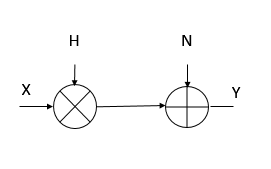
\includegraphics[width=0.95\textwidth]{fadingChannel.png}
	\caption{Power spectral density for a AWGN channel}
	\label{fig:AWGN}
\end{figure}

The Rayleigh fading channel before addition of noise to the signal is done, the signal is scaled with the fading coefficient. Also mentioned in chapter \eref{sec:rayleigh} and the corresponding equation \eq{eq:rayleigh1}.
\begin{figure}[!htb]
	\setlength\fwidth{0.8\textwidth}
	\setlength\fheight{0.4\textheight}
	\centering
	% This file was created by matlab2tikz.
%
%The latest updates can be retrieved from
%  http://www.mathworks.com/matlabcentral/fileexchange/22022-matlab2tikz-matlab2tikz
%where you can also make suggestions and rate matlab2tikz.
%
\begin{tikzpicture}

\begin{axis}[%
width=\fwidth,
height=\fwidth,
at={(0\fwidth,0\fwidth)},
scale only axis,
xmin=-4.50692133321182,
xmax=4.50692133321182,
xlabel style={font=\color{white!15!black}},
xlabel={In-Phase},
ymin=-4.50692133321182,
ymax=4.50692133321182,
ylabel style={font=\color{white!15!black}},
ylabel={Quadrature},
axis background/.style={fill=white},
title style={font=\bfseries},
title={Scatter plot},
legend style={legend cell align=left, align=left, draw=white!15!black}
]
\addplot [color=blue, draw=none, mark=*, mark options={solid, blue}]
  table[row sep=crcr]{%
-2.29096259197818	0.499525212628702\\
-2.07364859353226	1.84012863907324\\
-0.526187527043815	1.61306904215485\\
2.95741670892996	-0.527725084494009\\
0.622126647109399	1.85641553760022\\
1.10592216643447	2.51107063804871\\
-2.78150513390071	1.04684757069706\\
0.466225426531619	1.53293576536527\\
2.62986212504809	-0.720324220666362\\
2.27148765458696	-0.233438465754223\\
-1.30976397545005	-1.89044349391969\\
1.67965555368308	-1.89296994384237\\
-2.72684408006149	0.731940589108619\\
-2.94882169465128	-0.0595849021028069\\
2.43302760031072	0.51521947475285\\
-1.74826276512721	0.0322017495923453\\
-0.36061878282216	-2.31527952180523\\
-2.23967253555129	1.30443021600377\\
2.69393689613985	-1.9639943083955\\
0.256838297640955	-1.32567468821545\\
-0.0959242118368461	1.73607686412372\\
-1.22612532713436	-1.73424052557193\\
0.466470924917709	3.07746628934148\\
0.969966678093972	2.9907573411941\\
-1.89693873826648	0.842725045381543\\
2.20869370316849	-0.766951733381199\\
-2.49420836567618	-0.553424961465631\\
-1.265686333936	0.693359029540494\\
1.28455405789396	-1.96760317735738\\
-0.576924592819501	0.467811440987941\\
-2.84328835698185	1.17970465356548\\
-2.26414828367366	1.13170207080557\\
-1.21236459158778	-2.6073611423723\\
0.28214056879582	3.52788008260659\\
1.27930950004198	1.8697893506577\\
1.00865030898807	3.17820824028906\\
-1.63039652664464	0.772389322896464\\
-2.4873788600879	1.48770002437902\\
-1.9011955473152	0.582679866811802\\
-1.28219996198581	0.813586316639382\\
-2.03217371954866	1.87651780547952\\
0.287092745505636	1.3248822638822\\
-2.28332164983386	0.316774796838446\\
-0.704586291021065	-2.38284464830826\\
1.48467682000632	-0.465677824867176\\
1.02563816843502	1.6519776864232\\
1.56669768578929	0.480365557248015\\
1.33613563076523	0.574859636736496\\
0.682870141549008	1.05783086820108\\
-0.228738939218387	-2.32967559985497\\
-0.64873836944536	-1.65598325806027\\
-0.934953541917022	0.622662199740656\\
1.30830854664936	0.604173037656756\\
-0.040486734729829	-1.67925485816896\\
-2.79777572278367	1.31228015295939\\
-1.2235939903107	-0.202398397524856\\
1.75973262841731	1.74293204386269\\
-2.52533545460976	1.075964755706\\
-0.897998540188782	-1.64901604990939\\
0.744025481672709	1.16811813371144\\
0.374181542695076	-3.94717797934046\\
-3.08256344869877	0.627099468970679\\
-0.798593607461943	-2.63481744751108\\
-1.90752340702407	1.33870135675126\\
-1.70699939854124	1.98100781802658\\
-1.72428628282776	-0.00315290305219429\\
0.0823181174221582	-2.47562146347038\\
-1.80116072066558	-0.419620638462671\\
-1.72233221535843	-1.51594923211063\\
-0.229720394998758	-1.66443199862572\\
1.05476434466513	1.98135442141434\\
-0.785114446251288	-2.69346093710077\\
-1.9768232847583	0.180776779102788\\
0.213127461710832	1.59143788419485\\
-2.01345852587545	1.0743036759523\\
-0.599731673574226	-1.20971576815704\\
-1.13232137928996	0.547593717778279\\
4.01476276000414	-1.54823154587435\\
-2.18912283421444	1.87781682873093\\
-0.214428879109597	-3.3824585114223\\
-1.8610789098107	-2.81890196740714\\
1.42744541237467	-1.96616903871018\\
-1.63513246642466	-2.2398877191519\\
-0.661604026979681	-1.55308735742243\\
1.05159122216374	2.3404595486754\\
-1.90245403543523	-1.88866443886666\\
2.03096317384464	-1.01484150832954\\
0.796135918637663	2.22109636666806\\
-0.82567517136829	-0.671837787068517\\
0.197771368464553	2.01309279037339\\
2.49988154527328	-0.124018974984179\\
-2.43242992120185	1.67073460987441\\
-0.579929301371038	-2.76247917191727\\
2.06829804599968	-0.924133989935484\\
0.208272613507879	2.03896507815814\\
2.61429229769537	2.95311553638038\\
2.03122614592743	-0.835626407450464\\
-1.70455793105063	1.15852617221279\\
2.57298940710963	-1.47530118067478\\
2.07874983306073	0.913919151337478\\
-2.49427407559289	0.690845240760039\\
1.79279376222049	2.12505050908808\\
0.137185841025518	0.50191598510539\\
-1.95686982554467	0.888827551323542\\
1.28681065161923	0.0839077861445916\\
-1.50167775839181	2.26495031999906\\
-2.33466969647272	2.04288917361384\\
1.61539070864393	2.86723973855652\\
0.999189434262886	-0.917089263850896\\
2.93189064402613	-0.532575056267382\\
1.17602917386146	3.86098234209057\\
-1.32128000309466	1.06608143811188\\
-0.796767799778552	-1.83051821707545\\
2.40020554858777	-1.00412201309041\\
0.94918975372806	1.45691540363646\\
-0.92287179187706	-1.73885736100892\\
-2.80134429302997	0.57065690417674\\
-0.541021251900306	1.83719280455475\\
2.70801352286942	-1.40563598207446\\
-2.00015717257219	1.83330443818575\\
-0.233294935799565	-2.08751681049729\\
0.243804398724115	1.75302189121752\\
2.18095970445126	-1.41072148222887\\
-0.179491286583395	1.0792671753003\\
0.268808290730011	1.59937312042647\\
-0.0452191809424788	-1.80785415853454\\
-1.20692763655583	-1.51119628101661\\
-0.559473981045535	-2.3050381756176\\
0.875566258612658	1.88724323839101\\
-0.41651877226424	3.14912582806056\\
1.31418290015704	0.151563306513407\\
-2.63447264292101	1.20422018676871\\
-2.36638789739472	-0.0216333002834224\\
-1.11177635981107	-2.45264280173829\\
1.78605899238937	2.07135650093423\\
-1.57087686143634	1.48876360028291\\
0.730234529640452	-2.1722278220306\\
-1.32751587008845	-2.78104058940705\\
-0.130357031648477	-1.90263875083684\\
2.47803344775559	1.0667698111481\\
-2.08037243189072	0.893538234977945\\
-1.98611608545063	1.45263323903408\\
1.13016442046435	1.42917199387212\\
-0.380457453966021	-3.29088034966233\\
1.76237727894807	-0.970144521231341\\
-1.02733714034409	-0.858896883924002\\
2.47420713572839	0.701111492040435\\
-1.30448095998256	-1.70188755027961\\
-0.163686972675424	2.04669839673745\\
-1.87995032164349	1.28565746402464\\
1.36148385001257	-0.714125748125993\\
0.505418274483802	2.13624719858727\\
-2.54790005955721	0.868242236345207\\
1.98761836753389	-0.335969209276705\\
-1.77002509071918	-1.84522989782384\\
-2.23772121721848	1.05237103179119\\
-2.79470711559293	0.652891841397553\\
-1.9886240660243	0.327360905277998\\
-3.09308732207585	1.62633494506295\\
-1.88506695054411	0.1471298652799\\
-0.957365828029528	-2.05949583594659\\
2.21385259804759	-0.22204919140951\\
1.54754653847856	-2.26771648023671\\
-1.74096414501368	-2.10572785284077\\
-1.38847327388415	-2.29497122358013\\
-2.21844870576554	1.31449955046641\\
0.447897190847905	1.26862210509534\\
-2.96050935649553	0.811074807810027\\
1.0821804114983	2.47572191852441\\
-0.774247647824235	-1.58641746245712\\
-0.551046857020762	-0.540214748793858\\
-0.985760183976854	-1.5264374701882\\
1.70769127668423	1.39806604038147\\
1.48526002526875	-1.91235314214862\\
-2.8724089117701	1.50214990194036\\
1.15194672044809	0.131840491102762\\
1.65573555880715	-0.854509980054649\\
-2.32322104321157	1.19764662485124\\
1.31145785860626	-0.639319665644346\\
-0.436936801370411	-2.21468408463965\\
-1.27375145983165	-2.06179865121977\\
0.733056183537031	1.54513520238112\\
0.74164198452271	2.07578604005743\\
-1.65873043837377	0.356577924466779\\
1.72387573579859	-0.10396146977055\\
0.563122073780207	2.81000744678685\\
1.19241728533836	-0.65885180896336\\
1.53867861294664	1.87263096879716\\
1.78246450701243	0.749962766211448\\
-0.0320396623234895	2.17661709741632\\
1.44373003670696	-0.372027480639314\\
1.29093600206403	1.70452929630504\\
-0.355703903480474	-1.72513664320498\\
-2.08728856938777	-3.62041857697638\\
0.862197608127037	1.93575406167384\\
-0.598039686919064	1.06169554130377\\
1.67240862417181	1.63870190956959\\
-1.70910861908908	0.81818535355918\\
-1.46110414572735	-1.82715532689972\\
-2.69117556290707	0.292509181816015\\
0.116813525927179	-2.38823166638591\\
-1.09094009561679	-3.8729926366913\\
-1.5754587899603	1.38503983411467\\
-2.85586832719462	1.06215001848703\\
-0.777544082848482	1.48358518946647\\
1.18425650964166	1.9648203627014\\
-1.40044348925891	0.092619065677957\\
-0.542499110109995	1.5786375157017\\
0.0427107550304643	1.23685282476903\\
-1.88553628902867	-2.42393469831409\\
-0.876235006795336	-1.37931657241617\\
0.835057226437517	2.30737529854241\\
0.994030631042834	2.17784798177201\\
0.858995126203633	-1.11724598151498\\
-2.52275390600805	1.60435364787657\\
0.296743957091529	3.32639694300461\\
-2.07677094413645	0.586179597528627\\
-2.18977607133713	2.12884388798952\\
0.351432248430746	-2.06256541767101\\
2.21575759710432	-0.0340051680194582\\
1.98487765493515	1.6632503554187\\
-1.13109173221803	-1.43370345495467\\
-1.91975717529646	1.13021629883158\\
1.37165850602754	-0.807717658553789\\
1.00504476586126	-0.189430271325901\\
-1.10247519927924	-1.90353353625106\\
1.33825388538566	1.67067955881095\\
-1.4379051919646	-2.89886615686865\\
-2.05834775457136	-1.44080345380658\\
2.8053502453129	-0.895894550646062\\
1.79951160436875	2.61356069394257\\
-1.25301706293711	1.49415715373776\\
-0.890900512672852	-1.78524130171701\\
-3.08955933551945	-0.382139102819598\\
-1.34769388310619	-2.59260466456011\\
-1.34348462275602	-1.94681517931052\\
-1.02366945916322	-2.66546121049387\\
-1.53628037436969	0.541307466646004\\
0.653977445765453	2.33063990748991\\
-2.44978952812965	1.31537808814826\\
2.45265874098255	-0.385804522505506\\
0.824424519468446	2.15315406040132\\
2.97643277056973	-0.418914785590126\\
0.0885253807210014	-2.74354864575563\\
2.19116772775541	-0.201868726692018\\
-2.96032648761001	2.00739448676192\\
1.94048414649474	1.6768352520852\\
-1.03147502225348	-2.73026642369039\\
-1.48539284169198	0.174702340625983\\
1.3886514558579	2.07446273533694\\
0.153462151769068	2.17352789115303\\
1.12567964120882	0.538817557950431\\
2.89079770121188	0.171556416830162\\
1.95983709729105	2.83576782170002\\
3.02635267286194	-0.633100107722621\\
-1.31020352464299	1.93012516174761\\
2.97711407008144	-1.05058257512357\\
0.736940019312649	1.51941001300617\\
1.9486721801081	-1.34224306855365\\
0.0552567082732573	2.96054430573961\\
1.61583204626062	0.301447031571731\\
-0.150970148561366	2.15439509523647\\
-1.31061669425855	-1.61025255821996\\
1.55212313679985	-1.54058857266939\\
1.38039018111661	-0.136278821370928\\
-2.56732184533752	0.677066793580569\\
1.39143517390814	0.0654040366851971\\
1.08024286843312	-1.31752336546162\\
3.2306216514864	-1.05581539075352\\
1.77106993619275	-0.708655594850442\\
-1.3500673483192	0.638955003165831\\
0.408671879601026	3.20506492046067\\
-1.70812575343123	0.621155021721354\\
-1.56486044722244	-1.90876482754826\\
0.722707877478828	1.80297545166741\\
0.116081767358342	-2.41383830191321\\
1.94119581651736	-1.63677718629204\\
2.39503275534561	0.855805476470424\\
-0.538525166944102	2.17318217922565\\
-1.1075627703348	-0.547859263896077\\
-0.241950049946092	1.9217223318269\\
-1.10454942890708	-1.69033314515527\\
1.00230001736214	0.924180717579618\\
-0.879720226488485	1.75235374053969\\
-1.35090959192001	1.97411128758428\\
2.31783099534092	-1.63147130008429\\
2.81294727818487	2.20475308574013\\
-0.614798715554404	-0.9642025812877\\
0.257810196319554	2.08325970166155\\
1.41489484955119	2.86243729096327\\
0.280840460493608	1.02073078921305\\
0.960551664019401	1.91347685046647\\
-1.69579709155449	-0.0297459858288885\\
-2.94163531000485	-2.66992622506333\\
0.516239911335674	-0.435886442762418\\
0.785102571872502	2.0804676966826\\
-0.677816785613951	1.65184310142313\\
-0.806279435119176	-2.33308569173316\\
-2.0504411975335	-1.13380442942019\\
-0.945756770908074	1.21208607608518\\
2.20020926025892	-0.446375240110942\\
-2.8976332416704	-0.330138590946023\\
-1.70555557468702	-1.44386593234293\\
0.64487683890196	3.24122439384353\\
0.861482825414417	2.28476934524155\\
1.98464905678119	1.56909040968897\\
-3.03532081106956	2.59184366395308\\
1.87139898663515	-1.37377147927556\\
2.04116694108007	2.29725294293907\\
-0.17844534872087	2.42216911841678\\
-3.58348719788356	1.79634693270948\\
2.00509498798076	-1.01384606006658\\
2.98032654673437	-1.10668215692047\\
-1.49412359335905	0.766266686591987\\
-1.57926172382637	1.92326960456188\\
2.50770879860708	-1.04963693288523\\
-0.293314924226559	2.22414015289419\\
1.76706067657525	-0.191012912885881\\
0.258409864170699	2.08894254559685\\
-0.547306539665956	-3.20914235724389\\
2.29947060641309	-0.543020654285528\\
-1.13973068059764	2.25715938754058\\
-0.486779091215381	-3.03770321504317\\
-2.71855904104199	0.876969356273564\\
2.06225933618163	-0.629735067158132\\
-0.700292078227145	-1.20321027518341\\
-2.74483186957967	0.257387739798519\\
0.356054900875451	1.81114511491244\\
-2.49146962588193	0.296797138592803\\
-3.34326303206908	0.852097917887548\\
1.13259334241221	-0.839746658108864\\
-0.768927612299447	2.35162159663076\\
-2.1474959682315	1.64232788789786\\
-1.65347458683054	-2.43652574079159\\
1.42260756764987	2.76599136620879\\
0.940420736010442	2.03805948275817\\
2.21047234448016	0.419242278638436\\
-2.18957272814751	-2.87772401127464\\
0.817457895647391	1.22964471797792\\
0.375273545061793	1.67989484167706\\
3.33636531662061	-1.21440270505437\\
2.14374215093614	3.08584181203139\\
-2.33390796717999	0.754924383931941\\
-0.401645701994946	0.971757938712603\\
-1.55757775002553	2.1256392957874\\
-0.781721544196652	-2.63616142117176\\
-1.43625265175961	1.05254508627564\\
-1.62972478710597	-1.61403268189444\\
3.09264554341956	-1.67533000136533\\
-0.544145477332016	-2.9820462126652\\
-0.800104378809615	-1.03208712128695\\
2.46673201789136	-0.627977389759003\\
0.755633784838171	2.72296077182202\\
-1.29784260675854	-2.04502638266557\\
2.38536705535294	-0.611367186457392\\
0.0428210230515212	2.4875530990593\\
0.972458997151281	0.87943665659913\\
0.470047023524752	2.18867817883749\\
-1.19423328988103	-1.31321938600685\\
1.70392914340063	2.21138742631549\\
2.5033603700201	-2.17926436792457\\
-0.831169642000059	1.27978248828503\\
-3.72908227773688	-1.26730863501521\\
0.258609242047328	2.17025712266332\\
1.4917577004801	2.32645695826661\\
1.31679983761609	0.232141814195148\\
1.74710055863254	2.77393540301859\\
1.28360765777204	0.780725117039803\\
-1.31772322897619	0.262873009469883\\
-1.35256650063027	1.51175958710586\\
-1.32155903377318	-2.31687703858227\\
2.46958655296298	-1.55002441571576\\
-1.60022146499386	-0.536906084374203\\
-1.04973267937027	2.33871817699619\\
1.45966551515705	3.04844216618537\\
1.41418241865692	2.95618563817753\\
1.01387410392432	-0.583096698740427\\
-1.46884984498448	1.52844245151192\\
-0.922810525363503	-2.63557507504854\\
1.33582571243816	2.10737716050062\\
-0.758138523401223	0.95099580797654\\
-0.534304750818122	-1.86412502866636\\
-0.3650193186039	-3.14200959168648\\
0.747600894533258	1.77197660912749\\
2.78916169722755	-1.26521817936312\\
-0.988781699615665	0.5696017848383\\
1.17737268955883	1.80752441641451\\
-0.780498664800585	0.887162066533538\\
0.0899139321814095	0.234947568096862\\
-1.44215037626265	0.627935644815196\\
-1.33148253550327	0.674992664409848\\
1.67348922151854	3.05398587051633\\
1.11103348132601	-0.757040974587462\\
0.778517124605433	2.01373038644395\\
-2.92066968904276	1.25180313591785\\
1.65802652941974	2.85687478416805\\
-1.21528893462397	-3.05975830319484\\
1.58318223390117	1.01849394500332\\
-1.74889326528965	1.00777934706308\\
-1.90166166509362	1.19681948970579\\
-0.274692915163525	3.44652822468871\\
-0.740391131700495	1.35117535762659\\
1.47401435728733	2.10481897253824\\
2.38277180063857	2.28672421456904\\
-2.91119275164687	0.668024247902888\\
0.115166918644873	2.32680224858275\\
1.2359459917285	-1.40980854683391\\
-1.12199585416097	1.46666673620495\\
1.03163670538839	3.05639524582709\\
2.21325755747909	-1.78509240592948\\
-1.43296999633492	1.13593269683049\\
-0.366634182642934	2.22930278747331\\
-0.450915716656783	-1.03204222521495\\
0.988335771356353	1.50990514777502\\
-2.23173680222779	-0.40205411271176\\
1.94236803973783	1.12094960946529\\
-0.84448867983569	-2.08275357458644\\
-2.01314196299515	1.06302880635047\\
1.07217099364876	1.96013640922305\\
-0.467023353371759	-1.58997691648176\\
0.0264476009644421	-0.799873690685817\\
1.14431302503998	2.35359569118919\\
1.75992552282296	2.96745436757757\\
1.02369491818124	-1.3227499135541\\
2.49293947669924	-1.01814139626969\\
-1.70660580781328	1.72935387893255\\
-0.343520724881489	-1.47555327285638\\
1.99877166092918	1.45031808460054\\
-1.21221232770104	-1.76320474194217\\
1.03622438665108	3.57999320489096\\
1.40710851678528	0.681120154113882\\
-1.54520811065216	-2.16076896274386\\
2.31621050949727	-0.734135989718847\\
2.22962737892932	0.432102783028419\\
1.31311028433214	1.37956107422019\\
-2.61453675524317	0.0781623363907989\\
-2.56640837436955	0.455350707401279\\
2.91910214051456	-3.18346904337623\\
-2.51646646789714	2.34524172688287\\
0.303342837958312	1.55325826794405\\
1.78321469686914	0.453037909265406\\
1.32105484265208	-1.74089393673124\\
-0.824046533239037	-2.14941955981457\\
0.765222694753028	1.17703897875201\\
1.06716032113241	2.60006903314172\\
0.852399936395766	1.7902134313623\\
1.84942837351689	-1.23595411472555\\
-2.29226692346819	1.94490016707742\\
0.335259597741909	-2.18398889990501\\
-1.13437755725865	-2.46629059506871\\
-2.13118435577188	-1.93744894538773\\
-2.19985964967873	1.73404072389666\\
-1.59139346210064	1.48045188382733\\
-0.0734418166812236	-2.5509404142151\\
2.29252109515497	-0.813645461486738\\
1.75712390358607	3.8408325872367\\
1.796200550898	-2.78222601185603\\
2.43762531526232	-1.21731618488012\\
-0.966871531139459	0.561574349065999\\
-1.39356823277404	-0.873868577623283\\
-1.97227557411408	1.13571121746095\\
1.92306838657358	-0.525681794513612\\
-1.27222449798173	0.209968074048192\\
-0.519025763548393	-1.75124880026881\\
-1.65680204065669	0.455102480955756\\
0.0270620632337905	1.86082556362749\\
0.37562363315137	0.845423458709117\\
1.59560850432588	1.55621797610404\\
2.72045053506708	-0.227923170449448\\
0.572627704103753	1.54386244223983\\
2.18127132190865	-1.30077185800083\\
-2.47868937162692	-1.52118320802275\\
-0.766064880694681	-2.77959710767137\\
-1.80229232505761	1.43313993682003\\
-2.10361687637052	1.33786602808403\\
2.28978698045942	-1.38541835520804\\
-1.49506032792	0.863714191084605\\
2.5770358753371	-1.47633321213746\\
-0.258584211871664	-1.86920545509361\\
2.76627450760182	-1.44900785966452\\
0.958584123048307	1.12000258886451\\
-2.04167910719868	1.80533151323107\\
0.981242213541003	-1.17122797808903\\
-0.345721234784559	-0.421017634811581\\
-0.484274902905206	1.9989202331179\\
-0.493683281670055	1.20641037770084\\
1.65160663490717	-1.90062973894423\\
2.50288923764379	-1.47805642022303\\
1.72284714573192	1.44673140030518\\
1.75996623311519	3.75608811537522\\
1.95988426038479	-0.471479190869601\\
-0.00247563264545481	-2.10987093069313\\
-1.62898619734627	1.56903176627298\\
-1.0498652203383	-0.379705473581878\\
-1.97529853042249	0.549554155888005\\
2.87904847594672	-0.366669575113052\\
-2.37337826922358	1.23330161324718\\
1.05079480612811	1.19266358674046\\
2.22763889284374	-1.72125835674631\\
0.578710246050794	-1.3716677708642\\
3.63740692409208	-1.29112871694406\\
-0.0420286477817177	-1.98845815742357\\
-1.75537682817618	2.09108971213371\\
-3.19015382255872	1.77353101987891\\
0.887077597736859	2.37119404057864\\
-0.420619831547352	-1.80528733227946\\
-1.89262179301331	0.891520683354297\\
1.21691694616374	-1.99544556925536\\
0.874027809724726	2.94884094278122\\
1.47441290184152	-0.0783629810364507\\
2.23027767083616	-0.0781026755562821\\
2.07719020096037	-1.08555872376369\\
-3.00890273253385	0.910836288463723\\
-1.30573311023814	-2.40885837057242\\
1.09467457024389	1.03946953290944\\
2.58489579291233	-0.0295721256295831\\
-1.73380085721054	-2.55100063340654\\
-0.676062396648645	-3.21685907788583\\
2.26128623938087	2.53678747016712\\
-2.2215931995288	1.16464867539692\\
-2.37055477125933	1.17444081519014\\
0.688292831540016	-1.32441722676495\\
-2.28522069472459	-0.842762713743915\\
-0.232023405236719	-1.23905994717914\\
1.2876802410911	2.89448162894545\\
-1.20961654491217	-2.40965800812923\\
0.126804108496263	2.52455226006462\\
-1.0253490672465	-2.11878834372689\\
1.46755513184295	-1.92295951391194\\
0.721517609895742	0.781264553496529\\
2.7073884026703	-1.04040360535111\\
1.05616002810802	-1.16404648489516\\
-1.92234662709177	-1.80642556476037\\
2.22843520502463	-0.88966399313092\\
0.111908708187335	2.08371228487406\\
1.41589537706592	2.00532110749979\\
-0.451373126803023	0.390425593548175\\
-0.718930674877095	-2.35424611292123\\
2.25254351219649	-0.476186569441875\\
-0.730966381073949	-2.57879661278044\\
2.58082758957192	1.83586167439122\\
1.7301458091598	-0.211900974982417\\
-0.823286673527323	-2.9615691851014\\
-0.285779985841113	-1.62533837862207\\
-0.168994874351659	2.33959392839405\\
-1.20077840317802	0.85164930581402\\
0.921693286342653	2.75014821474253\\
-1.53603316516885	1.99068226671103\\
0.668746047634606	-1.27266587566376\\
-2.60506279136892	0.61230863813298\\
1.9966288510105	-0.960950617335661\\
1.66864441237384	0.123295974325853\\
-0.628980499066043	-2.02515957317547\\
-2.13503938595894	-2.1499028183484\\
-2.57326945562426	1.01349350317974\\
-1.02072022537704	-0.944625653349921\\
1.53172985835625	3.10095083643132\\
-3.47061469420119	0.719294622458664\\
-2.66746202343258	-2.0150860778732\\
0.367685832801467	0.734228624327285\\
-2.65340917952528	0.972918086791392\\
-1.43279206916743	-2.65239338129805\\
-1.54815548531387	1.04880384459015\\
-2.25490779595886	0.773599589828085\\
1.56980629738482	0.0219899037766047\\
-1.75694102264713	1.31814067736277\\
-0.416528716127031	-1.11319318188524\\
-0.84127169665838	-3.70687398121312\\
0.66291692478886	2.15037765544733\\
0.644339244247415	2.05246243303562\\
-0.56345899458864	-1.27612801772079\\
1.48838232777853	-0.924003542627079\\
2.80739103318104	-0.935892791422735\\
2.05914810674692	-1.85571257529125\\
-1.07165562917556	0.481947051905067\\
2.63420939625892	-1.47842421075874\\
-2.55844782436715	0.431113067174073\\
1.64088528757493	-1.15839690558582\\
-1.85771817077415	1.00472315587005\\
-1.18507233113866	0.34255578102457\\
0.719369497945252	2.41650730182583\\
0.812397189846	2.53229390526321\\
-0.253086950330635	-1.58661436065154\\
2.53483203201391	-1.51809149394841\\
0.452706306143167	1.4565877969314\\
-1.01183402695956	-2.58455840510877\\
0.273419453567819	2.32195707555838\\
1.05146220509014	1.85283057035905\\
-1.58517278208365	1.31665986694211\\
1.83383421748266	-0.868247538246099\\
-2.55476832599144	-1.85377507653468\\
-1.44411409785603	0.794083338733498\\
0.829180046422687	2.23760122757723\\
1.08342731035153	2.42676927720077\\
0.536215992618615	1.71470821571257\\
1.01085740227172	0.169645460793515\\
2.22514864975662	-1.93711784009953\\
-1.49732553225579	-2.40749831448581\\
-0.576152195597948	-1.70035951445631\\
2.02980065323139	-1.32733946678224\\
2.61499795198598	-0.840714865220088\\
-1.76301958031486	1.93151553168759\\
-0.937855333360853	-2.84970706567477\\
1.15925053430525	-1.70193061462212\\
-0.155464980572992	1.86743953289046\\
-0.92213843522521	-2.89416730635558\\
-1.55235505756812	0.86622182172128\\
-1.12330879747539	-1.98960940087248\\
1.08069627942787	1.89371232655967\\
1.59898057553315	2.74464477698829\\
2.31994509277003	0.567448772908772\\
-0.316687874159267	-1.46012588505221\\
2.92710161229141	-0.879180490710568\\
-1.65638621752076	1.41701188406866\\
-0.300115399069391	1.98503524864844\\
-2.14043419538653	1.09583611884894\\
2.87892348191801	-1.10104691670648\\
-0.679421858019839	-1.84898874387163\\
0.121256223921314	0.715601145555283\\
-2.29324272744951	0.760078976492137\\
0.530460905287272	2.28879350513664\\
-2.95718687564613	1.39870159304938\\
-1.14508817280496	1.08427187119285\\
-2.04365081764844	1.35890008608642\\
3.21732497735977	2.8720860964946\\
1.2302038015267	-0.356995792521685\\
0.519297155415213	2.30703820359795\\
1.33851774220825	1.9474391866439\\
1.02313379212009	-1.08989579220021\\
1.81353095910903	-2.46230978878501\\
-1.55665726499366	-2.8431339474276\\
-1.87832482969951	1.20888843999408\\
-2.91265540343494	1.35520905508617\\
0.177281562802525	-2.23303144363961\\
0.173398439566409	-0.101924133799895\\
-1.61108351178295	-3.0852813760866\\
1.67846083368305	-1.0298030737997\\
-0.951233346843022	-1.71686142254263\\
2.05143943144592	-1.21365091392369\\
1.00704459698345	2.03533115715963\\
-1.95798533072344	-2.4223532250787\\
0.863758017168416	0.435713025323596\\
1.94578636120917	2.66213508558544\\
1.75041267834482	-1.35763283634935\\
2.94615000095183	-0.370542023215318\\
1.05505669898112	3.38703401284801\\
2.24395092691407	0.866017051831697\\
-0.433206494166744	2.16184458815987\\
0.55904229806851	1.95634178576328\\
3.99834281643256	-2.17137218098499\\
1.26580471645021	2.23306868152319\\
-1.48330335175121	-1.54132627343875\\
2.0174900970751	-0.739100018925793\\
-3.46448198152898	-0.774367783504408\\
-2.13444545092344	0.151194952626948\\
1.3271745185255	1.89833289799892\\
1.18301261683367	2.11056906888564\\
1.44415024177114	-1.29487089953578\\
-1.13610849790723	-3.28867372243448\\
1.40385033698979	2.22049265188492\\
-0.24338786461042	0.773813852532025\\
2.64939927665201	0.452612826681451\\
-1.74247905399482	1.00991883815592\\
1.65129243790084	2.19274091698359\\
-1.08481137056571	-2.18233579502757\\
-2.4286495061362	0.62740899581501\\
-2.9520111193361	0.317186163917304\\
-0.380846699962743	-0.0253546476130552\\
-2.19459193282769	-0.515239816954554\\
-1.84765332261691	0.447671088806657\\
1.63019470398716	-0.727133990793644\\
-0.288462249249851	-0.755862161755658\\
2.273397182518	-1.55768388634932\\
2.19830378062083	-1.35401164366056\\
-0.841214843500358	-2.11385234226481\\
-1.70961752001437	0.760547665225515\\
-2.70673051379177	0.906366306937688\\
-2.67701042568905	1.44855895819788\\
-1.39364782642639	0.539670402436518\\
2.0517909243173	1.4123856390803\\
3.33200745226927	-1.06215843640997\\
0.392150270872964	1.85423775346743\\
-1.70756458503497	1.37637680296792\\
1.93504272504698	-1.27704585089434\\
-1.64245681363587	0.66445200223162\\
0.232173278617849	-2.46412908746548\\
0.330023254805233	2.58705181335283\\
-2.75730545966574	0.393356613945023\\
-0.343049650150252	-1.23946509887382\\
-0.747099469961489	1.76111305299882\\
-0.762365857936603	-2.61288198859131\\
-2.38034739533086	0.551421941784531\\
-3.05199566073061	1.40076887571126\\
1.77949544417258	-1.02989695378125\\
0.635362781360366	1.97810751678167\\
-1.32046310445302	1.16756594469327\\
-0.828075023945661	-2.33191331273006\\
-0.451016747463639	-2.25187009881915\\
-1.2333486609177	2.53769858942391\\
2.33827303143523	-1.08600819004904\\
1.72257398463698	1.83509059842472\\
-2.51884218181202	1.31012860368477\\
-1.67427534312039	0.985559759008651\\
-2.07039540244382	1.36081720677711\\
2.18484279696646	-1.62554828290516\\
-0.973722174431202	-1.38215915177673\\
-1.79673918919934	-1.92522094968014\\
-1.11758282831918	-1.17227116697743\\
0.519634851093578	-2.00247061107815\\
-1.52005832655128	-2.38141874095803\\
2.4020141453951	-1.56708065165772\\
2.77349348882212	-1.19870610293036\\
-0.426459153485832	-1.44044474008155\\
0.805240720473435	1.88051993832312\\
-1.37455541298112	-1.89859575054598\\
1.13293037080709	-2.43486419498477\\
-0.367429611451164	1.9783916644148\\
-1.6442206654945	1.42737454930168\\
-2.25505488793693	1.90146007704367\\
1.37610528060461	-0.0524049971307545\\
-1.39753951263515	-1.70627865269884\\
2.99476275737738	-0.529046343222386\\
-0.808436580789475	-1.40067206994412\\
2.91533095107974	-1.65161359736743\\
-0.971533466882928	-1.2434834739716\\
2.64902230409447	2.57050396093145\\
-0.635001391419698	-1.90287157780033\\
1.08169830653585	1.97094978121949\\
0.202244036415702	-2.931599312418\\
-2.37901378016889	0.578738127755981\\
2.06260793949653	-2.22653935458416\\
-1.18986040767568	1.01816156421674\\
1.55723020813949	0.210825632282545\\
1.02131857651834	2.39574938541474\\
0.189851942317302	2.70354234572578\\
1.05014107236126	0.00368144733828346\\
-2.09870814916299	0.253737248191675\\
-0.189308935277383	-1.75265207525351\\
-0.947352876892853	0.544713421210329\\
-2.63133886168298	1.70797279474105\\
-2.03040248921726	0.229380506501312\\
1.32250951271337	1.80873862159473\\
-1.25165551822426	-1.9831525623055\\
0.195201647599068	3.38253222750598\\
1.42188159211809	2.06552388827225\\
-1.11542860397525	0.780722179216293\\
-1.53432236232239	-1.86802562595029\\
-0.97162320720005	-3.31709583243601\\
0.761252624003148	1.53241861259695\\
-2.82099369006102	1.13087569510734\\
1.39743620955498	2.79357242110809\\
0.0732054373995167	1.14699238802469\\
-2.93589808266367	-0.19046602484409\\
2.06000774073951	-1.19136880350878\\
-2.53824494631547	0.769923185398166\\
2.62296024205509	-0.388954654236182\\
-2.97598031973617	0.212553289770989\\
0.617873501573524	2.70318999677884\\
2.43624088309919	-0.377918361588883\\
1.38142726727669	0.670115193804768\\
2.06659340648931	-0.0391706169581341\\
-1.5633392724062	-2.33400459683023\\
-2.64099096901911	-1.12467592981747\\
1.06616489835588	-1.09247910353194\\
1.71957082509865	1.81253244572585\\
1.5288156613977	-1.28038664167501\\
0.637763877312438	1.93076755785613\\
-2.15400950568792	-2.31517563545086\\
-2.43846653105863	0.919372633812635\\
-0.421408959708679	-2.08775431357491\\
3.01939420978803	-0.507564833605947\\
-1.40447132040689	-1.72616391459232\\
0.787447910266953	2.63046695827765\\
-1.28871562508812	1.91054293426122\\
-0.46949534393207	-2.58738518254937\\
-0.973753591206507	-2.68617766668404\\
1.51245110525805	-0.587033196216674\\
0.206201770415178	-0.762036993477668\\
-2.55475265754351	0.615286112774395\\
-2.90485677600928	1.48723188170248\\
1.21166299130586	2.26618576716768\\
-3.01458101258167	0.486070714635351\\
-2.41704801278966	1.03491192074624\\
-1.31601862673315	-1.36187245441692\\
2.42858083388929	-1.44021334910833\\
1.32974707752665	-1.42621855525423\\
-1.99905640761045	-3.13439426717514\\
-1.91429880332817	-3.16496817800307\\
-1.11944026537673	-2.00376185837925\\
2.10016356764288	-1.01223939219824\\
-2.72288444395627	1.58364791454769\\
-1.53875329646678	1.81944089075397\\
-0.0689629638909999	-1.6980735078273\\
0.214187275393372	2.21697004340992\\
-1.69140398425355	0.866138084337013\\
1.00514550748518	2.62675650352848\\
-1.07505815238699	-2.37928717038846\\
2.5115699245443	0.97902017238635\\
-2.34465250195142	2.74038793154229\\
-4.2120760123475	0.365711247197751\\
-0.647262951151161	-2.1385583586487\\
1.33495032717062	1.38062637165367\\
-1.94056532599375	1.89238299158861\\
1.86097385902193	-1.27342804905325\\
0.545515500215155	2.53909176512404\\
-2.27507928402971	0.64995917291711\\
-0.640630211267248	3.17918228096245\\
-1.59341984294926	1.75928959298612\\
-1.24266500675974	-0.789784801553393\\
-2.85062555797634	1.05916973978638\\
-0.703342099972954	-2.10556986268237\\
0.0858483325788292	-2.1267131120287\\
-1.05521052633119	-2.66798730398367\\
-2.00727605040034	-3.38039443077737\\
0.353217814677678	2.45411278611749\\
-2.26679244113664	0.223749161564134\\
-0.675954707579567	-2.90489488404116\\
1.95624213642495	-0.991906934551111\\
-2.07572241096689	1.09943359797551\\
2.13608587252859	-1.20869177301881\\
-2.67725340719102	0.74677870297589\\
-0.57582886585615	-1.04624493581618\\
-1.96542215285281	0.812127975603023\\
-1.22676381128582	-0.284892680175645\\
2.64547569737579	-1.38873265078063\\
-0.199867385804634	2.52906518142325\\
0.461692064203469	2.49168468736648\\
-1.32346943632302	-1.90531677439924\\
-0.150276816578401	-3.0618164452552\\
-1.78821189492221	1.96245617518577\\
1.90676430829506	1.56124415994945\\
1.19130915008417	-0.483471347055335\\
-0.832486334569584	-1.95778986788428\\
-0.306417178811679	0.33460742293934\\
1.64792178584984	2.30683475240532\\
0.86410517224765	1.5845642127029\\
1.94813530339064	-1.39517277745865\\
2.80276729232002	-0.778609438372601\\
0.984760908924227	1.55738316874718\\
-0.587123971895285	-2.39543692471356\\
2.87308671632232	-0.772560879850872\\
-1.82933423395299	1.06384327832438\\
-1.32789732050769	0.377435508638012\\
-2.35416247124355	1.83955392320923\\
-1.65081024472137	0.680638433530714\\
-0.193534891883996	-2.78487160774926\\
1.27094248643312	-1.46226413160612\\
1.94513197084025	3.36363126221259\\
-0.346415471449889	-2.3685163433018\\
1.17738839331607	2.50171504993536\\
-1.06727086461651	-1.16053796963654\\
-1.72109075309988	1.72758515658874\\
-0.0523960793876873	-3.06443012854533\\
-3.18440163906581	0.192232664238258\\
-0.589677870034226	-2.49671097934354\\
1.52407388063496	2.10333498367049\\
2.57790285110547	-0.568273623682279\\
1.92657736620926	2.39634313755211\\
1.58130579634579	2.32857795261866\\
-1.94880688076185	1.29340206018387\\
-0.961465426066925	-1.53740113778063\\
2.58830403965371	-1.55691606203199\\
0.723303653519752	2.34525943227863\\
-1.99179288867083	1.29263072017808\\
1.73602634694272	-0.665846164899523\\
-1.15682682414322	-0.78343953997859\\
-2.37511036602481	0.728412884725227\\
-0.0329037148504326	-2.688814574421\\
1.35064618880586	-1.48762423334738\\
1.83586030361568	1.64832651798747\\
-1.86061743000455	-2.28189051990859\\
-0.732218019353603	0.258167393094657\\
-1.7428587987218	-2.16845209963701\\
-2.69172741098979	1.22087508562651\\
-1.79329947937785	-1.83058146203777\\
1.02764709002714	1.69947722740741\\
0.138427394528049	1.40343468112249\\
1.57959108771354	0.904528643874035\\
-0.602360670476746	-1.3232646252726\\
2.12970401027251	-1.80694508221867\\
0.656008288933676	1.21087384218814\\
0.22247557077405	2.09632465371181\\
0.9444630251994	-1.39021257344605\\
-2.76041972429668	1.12254971369912\\
-2.15444629695636	1.10575317637665\\
1.50549222655156	2.21511222562903\\
2.29958130327429	1.92619351107014\\
0.151840410361659	-1.6844429027037\\
1.77940469244046	-0.508666777601648\\
-2.26625803319587	-1.67707946026544\\
1.50201521143182	2.10428340014765\\
-1.34364702575719	0.155820155429086\\
-1.99861986663313	1.92273621268066\\
-2.08515514615518	1.66948613909519\\
0.888752851083171	3.38126514278761\\
-1.69199705650597	-1.66512517700661\\
-0.84205399454864	-2.4028512952158\\
-0.510555218361393	-1.45191852894113\\
-1.3278481864377	-1.96582421499222\\
1.83591011551201	-1.83846958103347\\
0.567281413795519	-1.04586242906013\\
1.99517509446555	-0.0899700093108849\\
1.75906977256401	-1.71007773026698\\
-2.73454645528459	0.542514006718949\\
0.952008590318133	1.43962424211289\\
1.26013852733203	1.48400183812879\\
-2.74399605190792	1.69304984763642\\
-0.399961236369266	-0.98364030234671\\
-3.49980494991863	1.07923524548525\\
-1.81745652166805	2.49952866321411\\
1.63866413519061	2.38189898681835\\
1.01730423342752	1.76453047479335\\
0.717460027168265	1.81682361742157\\
2.91933516274331	-0.672365152363195\\
-1.80921568640679	1.66094545792883\\
1.5300032692546	2.65826814318341\\
-2.42980890548107	0.726275767985623\\
0.723355626895071	-0.70939629632012\\
1.12584955154988	2.4182757925128\\
-2.05941841316401	1.52355535166406\\
-1.57281079224839	0.061445726197766\\
0.897235351048522	-2.59921829550499\\
-1.67488434344298	0.969304523010127\\
0.119069029031057	2.57067433857838\\
-0.828088285861333	1.26252285555765\\
-1.01872295077544	3.26387642889065\\
0.806621075462451	2.02568262107454\\
0.655397722962797	2.33713776835214\\
-1.41736235529796	2.12318615235771\\
0.70937473503614	-1.26654142121455\\
1.31821885083005	1.40022203462343\\
-0.114207356526537	-1.95182008448425\\
-2.20074276033073	0.215234229463288\\
-0.790364530128135	1.83057647664771\\
0.987140785227774	-1.1345232161428\\
-1.92792705185817	0.396515605140828\\
0.422256576469073	1.61225302919008\\
0.278940008958491	3.21834191725988\\
1.87484462045803	-0.227598016375583\\
0.781499495593474	-2.6788391628052\\
0.320622524964136	-2.19833076244219\\
1.86691292342612	1.56910598203229\\
-1.69366886814647	1.53414845426116\\
0.840099089850138	-0.888650906099787\\
-0.657294245886585	-1.35562605597859\\
-1.33571864175259	1.71030114419912\\
0.596682054210849	2.06494562403294\\
0.0465719148527292	-1.61401038581647\\
0.88877232939587	2.27651777331845\\
-1.71224211513411	1.41864477493961\\
-2.28286402455753	0.504316089313754\\
-1.01015967749713	-1.59964868420161\\
3.07990379312002	0.209565725309292\\
2.23191774519887	1.64243558805428\\
-0.471136226318736	-2.51189981567748\\
1.96505742958463	-0.898455634687912\\
-0.597810049282849	0.943289744169025\\
1.00485656011646	2.31073403978039\\
-2.99835389675433	0.0545443757851337\\
-1.69117783357613	0.503458816446034\\
-2.21038906361543	0.803607849814609\\
-1.11286809135256	-1.54884561355233\\
-0.401883708073092	-2.51744751567411\\
-1.59179716087127	1.23719898761643\\
0.834121622017643	2.2744931640219\\
-1.24784664574969	1.51218960279631\\
-1.82472270109886	0.303876780954876\\
-1.52922490474279	-1.575319747838\\
0.237494716204784	3.02274691765921\\
1.7532887324881	0.0310049058966091\\
-1.70722608941292	0.485698516724383\\
2.28676697939932	-1.28022410742637\\
-0.599994944642582	-1.83374663929197\\
-2.21591801213829	-2.09525459217966\\
-2.08481482420468	-2.26185069401488\\
0.511836745193486	1.48458247452926\\
-0.154377220468614	-2.34757676095236\\
-1.4287227734863	1.40536215003517\\
2.43965215024944	-1.0243094659547\\
0.762261354683829	1.56105329326638\\
-0.969455899416252	-1.61437916176716\\
3.67521456361088	-0.965638535505166\\
-0.0194467804611096	1.94789229196469\\
2.39594595616272	0.484488170242301\\
-0.420469192728826	-0.577222264924699\\
1.73835566837631	1.610017715798\\
0.104191080016397	-2.29575674866017\\
-1.7932185220541	-3.56918984637673\\
2.33719216947092	-1.03950323000907\\
1.59553295629553	-1.34396963506183\\
1.70387580328551	2.16744814579096\\
0.0896445938163609	-1.56130675175906\\
1.12817137296995	1.26029712000396\\
-0.602251970018991	-2.9449147621178\\
-2.37949281979243	1.31630945212779\\
1.88915795066416	-0.838358650484433\\
-2.14931248611401	-2.30666547895946\\
0.388179610521463	-2.41699227385109\\
-1.39519500801148	0.307908243748297\\
-2.459851573324	1.04626904429342\\
1.17707466432488	1.77117102448305\\
-3.00826413503208	1.13830557900781\\
1.44452201810792	-1.21088820024611\\
-1.69046085318449	2.03225576867717\\
-0.554912080264299	-1.23860997612503\\
1.95173206426194	-1.60881937292678\\
-2.42250811627149	0.774533872531321\\
-2.25875883475146	1.22092377152983\\
1.49378528776602	2.19828946258032\\
-1.46520561627499	0.659379650818824\\
-2.63492648175126	-0.257096746442977\\
-3.4198327961416	0.84264034318562\\
2.96557953017861	-0.195024798912799\\
-0.998277883059853	-1.92000469993667\\
-3.28864504575276	-3.10702194474092\\
-1.96727621237205	0.607382598750473\\
0.494127246434622	2.12560859329597\\
2.66291875265036	-0.8807129941357\\
2.53316749880727	-1.39389664814899\\
-1.61753875030944	0.896793307652334\\
-2.11317437061595	0.173218546172624\\
-1.32879278508123	-2.41807122934347\\
1.64131476006099	-0.0697120151956349\\
-0.535976392638827	1.45991438804802\\
-2.32219428895032	0.0396719793029385\\
-0.608276474178876	0.742252152670117\\
-1.51340071635131	-2.32425069105161\\
-1.18882679953943	0.763473732370756\\
-2.32842770566053	0.580189130765605\\
-0.782691119428171	-2.13311883614938\\
-2.45466653571808	0.458520509672862\\
2.20332074478051	0.201738288612821\\
-2.15150842961423	-2.70872512343132\\
-3.67392258968944	1.76230920199615\\
1.99125552548137	-1.79096410913482\\
3.15428728051035	-1.41276264934725\\
1.55111891671804	2.88241067323069\\
1.76311249851176	2.66993037296282\\
2.55364990650353	-0.843533888698944\\
1.52431198455639	0.98459306090767\\
0.850892560276273	2.28247964294095\\
-1.07425568358916	-2.72627988228694\\
-2.17116252679267	0.588844119692995\\
-1.44249885009052	1.73873182359138\\
-0.966767948272623	-0.434197131235993\\
3.114527852011	-1.55241758519908\\
-2.11717803746428	0.856637841846722\\
2.16569397673932	-1.1028923918771\\
2.67947492148925	-0.386088473873236\\
-0.780032313515729	-1.6289982097728\\
-0.789716570777764	0.370014065807776\\
-1.26695288553955	-2.91730729758735\\
-2.01559763887338	0.143619104326064\\
-2.01130405555595	-3.00389422170674\\
2.52336961309368	-2.09399327903129\\
2.98798844467756	0.0108247982405226\\
-1.71438906651945	1.59776815257836\\
-1.63210494378588	-2.32333695936805\\
-1.862371248834	-2.45168649454378\\
-0.579252370403307	1.74436226934065\\
-0.389492006095497	-2.6337729085687\\
-1.60334631695319	1.66328989023254\\
-1.93432104058752	-1.82101061450591\\
2.1446059316122	-0.548524986573193\\
0.866841682085618	1.37912326733262\\
2.56623702195592	-0.338815438407311\\
-2.05921566599283	0.39909333676905\\
2.55010055733501	-0.447917024043323\\
1.26497287072498	3.15416408474838\\
0.9412018703431	-1.90034023745033\\
-2.26559526212715	1.03157076406484\\
-1.38900915092257	1.73765235574776\\
-1.35805068303804	0.0835767347001494\\
-2.29557279417698	0.412834893562717\\
0.393428343163375	1.08937129583175\\
1.34336462742109	-0.539496701079147\\
-2.58531135048289	0.958343982755532\\
1.78381951540891	-0.744713228956138\\
0.720681448572303	2.59927611871782\\
1.89410704879541	-0.121819023063272\\
2.77315108882483	-0.773650579094794\\
-1.51859874701221	-2.67139794088018\\
2.73775355666863	-2.19956530166046\\
1.09359034858342	2.54745859128982\\
-1.41025458697169	0.69451947662517\\
-1.72919879346993	1.50216796741261\\
1.70850634618917	2.68283905484481\\
1.8226477398315	-0.45257275448833\\
0.769722903817649	3.05377114191903\\
-0.87731636176603	0.328370947663204\\
1.40598113823853	2.37547232235967\\
-0.658672540187024	-1.76100468190777\\
-1.66534420997374	-1.68368646091488\\
1.89425591049337	-0.502907480532963\\
-0.323083868286948	1.88115414118976\\
-2.29219771643846	0.648423287959853\\
0.592855386892615	1.55008727104668\\
1.06674007593429	1.92527494426424\\
3.57317395834115	-0.114959935010961\\
1.09506141847865	2.09458441769495\\
1.96981692642768	-0.683291232958622\\
3.33393283563207	-0.460703136798398\\
2.7809035418368	-0.49477950028351\\
1.01768659615194	1.13896421764235\\
2.2738113367296	-2.48105044828011\\
1.59113756446148	1.44761594139921\\
0.103802719650948	-1.72150656564069\\
-3.5118111944838	-2.93526930210658\\
2.07240244682127	-1.70153849428496\\
1.08580867437802	-0.078606037428772\\
-2.49616522820547	1.43480531596362\\
2.22608091364862	-1.07565059792974\\
0.456384270485069	1.91355820689867\\
-0.280282423366797	-2.24118356847518\\
2.03010566613729	1.9167831040277\\
1.27946425410444	3.03565670039561\\
-0.455127841637476	-2.0012857734257\\
1.79111418851189	0.223414005332674\\
0.554765503106636	1.68748488117654\\
1.69950232436867	3.09486470049842\\
0.170462096524999	-1.15947178923294\\
-0.122260623806242	-2.78281229304992\\
1.28211369407779	1.77852248780369\\
0.487039922044465	0.870211251810638\\
-1.54147695835599	1.15920069594651\\
1.96009735963082	0.861888039576188\\
-1.26296808228541	0.108461707026283\\
0.13460411424659	2.42798427101673\\
-2.79340554730969	-0.919129997539706\\
-2.03584031372268	2.19125487993851\\
-0.233144973700432	-0.924988730068754\\
-1.53589556733908	-1.8546948980512\\
-2.25701346822282	0.484110598083343\\
-1.8645833140394	1.97079051840988\\
-1.74604624253968	1.98460076292195\\
2.70063273164032	-2.10723078917488\\
2.57189018352801	-0.845058623350515\\
-0.405987037181998	1.74462938491884\\
-2.04626068234686	0.873426132378649\\
-1.02934804401319	1.21953500794146\\
1.3637237985295	1.24505163987957\\
-0.0620320527024492	-1.24611410455152\\
-2.78488807435396	0.927978650991723\\
1.36237890158908	2.04182982316878\\
1.63098277645099	-0.784347041356602\\
2.00445965109213	-1.57359072788688\\
-1.93339627733259	-2.64848879416569\\
-0.593052962914238	-2.03011256277214\\
1.4883048860068	-1.54873234112639\\
1.47754376177624	2.44587645283028\\
-2.27012895538201	1.52967424604575\\
1.49436450841201	1.69675521525959\\
0.269511472917138	0.138528177500063\\
};
\addlegendentry{constellation points}

\end{axis}
\end{tikzpicture}%	
	\caption{Scatter plot for constellation points with Rayleigh fading in I/Q-plane.}
	\label{fig:scatter}
\end{figure}
As seen in \fig{fig:scatter} with various fading coefficients the overall power of the signal can increase or decrease, which also results in a bigger/lesser interference of AWGN noise. Still it is important to know, while higher "power" is beneficial for the error probability in the system it is not needed to maintain stable information rate. At the same time a decrease in "power" will make the system suffer a loss in information. So in the end it is from utmost importance to try and reduce the fading from the received signal $\boldmath\underline{Y}$.
\clearpage
\section{Receiver CSI}
We will now discuss recovering the signal with perfect channel knowledge. The received symbol Y has these properties: 
\begin{equation}
\label{eq:raychan}
\underline{Y} = H * \underline{X} + \underline{N}.
\end{equation}
With the knowledge of the fading coefficient a simple division of the equation will solve the problem.
\begin{equation}
label{eq:raychan2}
\underline{\hat{Y}} = \underline{X} + \underline{\hat{N}},
\end{equation}
with $\underline{\hat{Y}}$ being the new estimation of the received code word and $\underline{\hat{N}}$ the division of the noise with the fading coefficient.
Although the fading has been removed from the initial sent code word the restored code word \textbf{$\underline{\hat{Y}}$} has still to be considered a fading channel because of $\underline{\hat{N}}$. It is expected that this channel has a decrease in performance in comparison to a normal AWGN channel.

\section{Fading Estimation with Pilot Symbol}
In this section the scenario is taken into consideration that the receiver does not know the fading coefficient, but still has the information of fading block length. Now a method of restoring the code word \textbf{$\underline{X}$} has to be found.
\newline
One common and simple method used is the addition of pilot symbols into the codeword \cite{Hassibi03}. To the code word additional pilot symbols will be added. In this simulation only one pilot symbol per block has been added. 
\begin{equation}
\underline{X} = [X_p, X_1, ..., X_N]
\end{equation}
The pilot symbol $X_T$ has a set constant value both known at the transmitter and receiver side. With this knowledge an easy estimate can be given for the fading coefficient for each block.
\begin{equation}
Y_p = H * X_p + N
\end{equation}
\begin{equation}
\hat{H} = \frac{Y_p}{X_p},
\end{equation}
being an estimate because of the unknown portion of noise. With an increase in transmission power an increase of accuracy in the estimation of $H$ can be given.
A recovery of the received signal \textbf{$\underline{Y}$} with the estimate {$\hat{H}$} will be done. For this we apply the same done for receiver CSI by taking the estimate \textbf{$\underline{Y}$} as true value and dividing again.
\begin{equation}
\underline{\hat{Y}} = \frac{H}{\hat{H}}\underline{X} + \frac{\underline{N}}{\hat{H}} \textrm{, with } \frac{H}{\hat{H}} \approx 1. 
\end{equation}
It is to be expected, that this method will result in a worse performance than the recovery with the receiver CSI.  

\section{Simulation Results}
This section will discuss some cases simulated in this thesis. We will differentiate between different block sizes.
\begin{figure}[!htb]
	\setlength\fwidth{0.8\textwidth}
	\setlength\fheight{0.4\textheight}
	\centering
	% This file was created by matlab2tikz.
%
%The latest updates can be retrieved from
%  http://www.mathworks.com/matlabcentral/fileexchange/22022-matlab2tikz-matlab2tikz
%where you can also make suggestions and rate matlab2tikz.
%
\definecolor{mycolor1}{rgb}{0.00000,0.44700,0.74100}%
\definecolor{mycolor2}{rgb}{0.49020,0.18039,0.56078}%
%
\begin{tikzpicture}

\begin{axis}[%
width=0.951\fwidth,
height=\fheight,
at={(0\fwidth,0\fheight)},
scale only axis,
xmin=0,
xmax=50,
xlabel style={font=\color{white!15!black}},
xlabel={SNR in dB},
ymode=log,
ymin=1e-05,
ymax=1,
yminorticks=true,
ylabel style={font=\color{white!15!black}},
ylabel={FER},
axis background/.style={fill=white},
title style={font=\bfseries},
title={FER vs SNR for one block fading},
xmajorgrids,
ymajorgrids,
yminorgrids,
legend style={at={(0.1,0.1)}, anchor=south west, legend cell align=left, align=left, draw=white!15!black}
]
\addplot [color=red, draw=none, mark size=4.0pt, mark=asterisk, mark options={solid, red}]
  table[row sep=crcr]{%
20.973	0.01\\
};
\addlegendentry{FER reaching 0.01}

\addplot [color=green, draw=none, mark size=4.0pt, mark=asterisk, mark options={solid, green}]
  table[row sep=crcr]{%
30.728	0.001\\
};
\addlegendentry{FER reaching 0.001}

\addplot [color=mycolor1, line width=2.0pt]
  table[row sep=crcr]{%
0	0.735294117647055\\
0.345006900138003	0.681038527264935\\
0.665013300266004	0.630714501403254\\
0.962019240384805	0.584007514900386\\
1.00902018040361	0.578222010599916\\
2.01104022080442	0.597767353641397\\
2.48104962099242	0.553703083981233\\
2.91705834116682	0.512826442339044\\
3.02706054121082	0.501223761848978\\
3.28906578131563	0.464172515773549\\
3.53207064141283	0.429808192123438\\
3.75707514150283	0.397989373928894\\
3.96607932158643	0.368433227250407\\
4.00708014160283	0.363608580216078\\
5.01410028200564	0.35865736068949\\
5.36810736214724	0.33217340236862\\
5.69611392227844	0.307634593528946\\
6.00012000240005	0.284890737332231\\
6.26512530250605	0.26380652454365\\
6.51113022260445	0.244234010030475\\
6.73913478269566	0.226093630725583\\
6.95013900278006	0.209305823561846\\
7.01314026280526	0.204898380234375\\
7.46414928298566	0.189781683960414\\
7.88215764315287	0.175771087413817\\
8.14116282325647	0.166824754853019\\
8.48916978339567	0.154506819572921\\
8.81217624352487	0.143073793436507\\
9.05918118362367	0.134971635892549\\
9.46518930378608	0.124996493538924\\
9.84119682393648	0.115758430669558\\
10.5062101242025	0.100230222352396\\
10.8292165843317	0.0928114311726949\\
11.0182203644073	0.0888186516564796\\
12.0092401848037	0.0848467411701339\\
12.3182463649273	0.0785840590802866\\
12.6052521050421	0.0727672637411723\\
12.8712574251485	0.0673760875732125\\
13.2692653853077	0.0596001784054835\\
13.4992699853997	0.0551868529069559\\
13.7122742454849	0.0510997297278851\\
13.9102782055641	0.0473004321248046\\
14.0112802256045	0.0455304518020051\\
14.7932958659173	0.0421750887031978\\
15.0183003660073	0.0411077240557101\\
15.3263065261305	0.0380703471911418\\
15.6123122462449	0.0352499258168997\\
15.8773175463509	0.0326365983197871\\
16.0313206264125	0.0312416687636611\\
16.4213284265685	0.0289366984197038\\
16.7833356667133	0.0267972131260818\\
17.1443428868577	0.0246755122157184\\
17.4573491469829	0.0228513748630269\\
17.7473549470989	0.0211612795522263\\
18.0573611472229	0.0194839706631259\\
18.4603692073841	0.0180440713518843\\
18.8333766675334	0.0167113605749779\\
19.0303806076122	0.015977235836242\\
19.2893857877158	0.0147939211117418\\
19.5293905878118	0.0136974132589231\\
19.7513950279006	0.0126831434950658\\
19.957399147983	0.0117419742547299\\
20.0114002280046	0.0115292611535355\\
20.547410948219	0.0106790449146781\\
21.0034200684014	0.00995185961252762\\
21.2744254885098	0.00921557190053592\\
21.5254305086102	0.00853362276507495\\
21.7584351687034	0.00790057834849167\\
21.9744394887898	0.00731372172195958\\
22.0094401888038	0.00723961875956466\\
23.002460049201	0.0067473293843811\\
23.3534670693414	0.00624828273188751\\
23.6784735694714	0.00578620249809708\\
23.9794795895918	0.00535824511234034\\
24.0744814896298	0.00520988247093649\\
24.3154863097262	0.00482421902938536\\
24.5394907898158	0.00446576006296429\\
24.7464949298986	0.00413450557167341\\
24.9384987699754	0.00382725502902684\\
25.0105002100042	0.00372425725582354\\
25.6395127902558	0.00344979857142491\\
26.072521450429	0.00327510087535394\\
27.002540050801	0.00305083451392906\\
27.3455469109382	0.00282551611594386\\
27.6635532710654	0.00261662034171855\\
27.9585591711834	0.00242283338135229\\
28.0395607912158	0.00236348273027635\\
28.2555651113022	0.00218805911689864\\
28.4555691113822	0.00202562984525262\\
28.6405728114562	0.00187538276898007\\
28.812576251525	0.00173569359536447\\
28.9715794315886	0.00160656232440588\\
29.007580151603	0.00158177833653467\\
29.5265905318106	0.00146518900088966\\
29.9995999919998	0.00135893320944441\\
30.0566011320226	0.00132777819748156\\
30.2366047320946	0.00122898441814906\\
30.4036080721614	0.00113732574510171\\
30.5586111722234	0.00105225332400984\\
30.7016140322806	0.00097376715487348\\
30.8346166923338	0.000900769529033364\\
30.957619152383	0.000833260446489507\\
31.0046200924019	0.000810231004620098\\
32.0026400528011	0.000859313586271726\\
32.2476449528991	0.00079561231224624\\
32.4746494929899	0.00073659113182264\\
32.6846536930739	0.0006819900398008\\
32.8796575931519	0.000631289025780512\\
33.0116602332047	0.000599533590671813\\
34.0006800136003	0.000559823196463931\\
34.1616832336647	0.000517962359247183\\
34.3106862137243	0.00047922158443169\\
34.4486889737795	0.000443340866817334\\
34.5766915338307	0.000410060201204025\\
34.6956939138783	0.000379119582391644\\
34.8056961139223	0.000350519010380205\\
34.9076981539631	0.000323998479969598\\
35.0067001340027	0.000300134002680055\\
36.0017200344007	0.000319862397247943\\
36.2977259545191	0.000296181923638473\\
36.5717314346287	0.000274261485229705\\
36.8257365147303	0.000253941078821576\\
37.0607412148243	0.000235140702814055\\
37.2787455749115	0.000217700354007079\\
37.4807496149923	0.000201540030800617\\
37.6677533550671	0.000186579731594632\\
37.8417568351367	0.000172659453189064\\
38.0137602752055	0.000159862397247944\\
39.0017800356007	0.000149857597151943\\
39.1417828356567	0.000138657373147464\\
39.2717854357087	0.000128257165143303\\
39.3927878557571	0.000118576971539432\\
39.5047900958019	0.000109616792335847\\
39.6087921758435	0.000101296625932519\\
39.7047940958819	9.36164723294464e-05\\
39.7937958759175	8.64963299265988e-05\\
39.8767975359507	7.9856197123942e-05\\
39.9537990759815	7.36960739214778e-05\\
40.0028000560011	7.00560011200221e-05\\
40.2758055161103	7.55161103222067e-05\\
40.5698113962279	8.13962279245589e-05\\
40.8868177363547	8.77363547270945e-05\\
41.0048200964019	8.99035980719615e-05\\
41.3368267365347	8.32634652693048e-05\\
41.6448328966579	7.71033420668416e-05\\
41.9298385967719	7.14032280645607e-05\\
42.1938438768775	6.61231224624489e-05\\
42.4388487769755	6.12230244604895e-05\\
42.6658533170663	5.66829336586734e-05\\
42.8758575171503	5.24828496569932e-05\\
43.0098601972039	5e-05\\
44.0138802776056	4.98611972239445e-05\\
44.3818876377528	4.61811236224725e-05\\
44.7228944578892	4.27710554211084e-05\\
45.0059001180024	4.01180023600474e-05\\
45.1639032780656	4.3278065561311e-05\\
45.3339066781336	4.66781335626714e-05\\
45.5169103382068	5.03382067641355e-05\\
45.7139142782856	5.4278285565711e-05\\
45.9259185183704	5.85183703674072e-05\\
46.0069201384028	6e-05\\
47.0039400788016	5.98423968479372e-05\\
47.1169423388468	5.53223064461291e-05\\
47.2219444388888	5.11222224444491e-05\\
47.3189463789276	4.72421448428966e-05\\
47.4089481789636	4.36420728414571e-05\\
47.4929498589972	4.02820056401125e-05\\
47.5709514190284	3.71619432388644e-05\\
47.6429528590572	3.42818856377125e-05\\
47.709954199084	3.16018320366407e-05\\
47.7719554391088	2.91217824356487e-05\\
47.829956599132	2.68017360347209e-05\\
47.8839576791536	2.46416928338568e-05\\
47.9339586791736	2.26416528330567e-05\\
47.9809596191924	2.07616152323047e-05\\
48.0009600192004	2.0009600192004e-05\\
48.1579631592632	2.15796315926318e-05\\
48.3269665393308	2.32696653933079e-05\\
48.5089701794036	2.50897017940361e-05\\
48.704974099482	2.704974099482e-05\\
48.9159783195664	2.91597831956641e-05\\
49.0029800596012	2.99701994039881e-05\\
49.22498449969	2.77501550030998e-05\\
49.4309886197724	2.56901138022761e-05\\
49.6219924398488	2.3780075601512e-05\\
49.7989959799196	2.2010040200804e-05\\
49.9629992599852	2.03700074001478e-05\\
50	2e-05\\
};
\addlegendentry{FER perfect channel}

\addplot [color=mycolor2, line width=2.0pt]
  table[row sep=crcr]{%
0	0.892857142857142\\
0.663013260265203	0.827082017830828\\
1.02702054041081	0.789526779546583\\
1.40902818056361	0.73122280516428\\
1.76303526070522	0.677192420527287\\
2.01304026080522	0.641785562983991\\
2.86705734114683	0.691553458108793\\
3.01406028120562	0.698201428737776\\
3.67207344146883	0.646756191867099\\
4.18808376167524	0.609370527394584\\
4.90709814196284	0.564461755941113\\
5.05610112202244	0.553656363866127\\
5.51411028220564	0.512813099391532\\
5.93811876237525	0.475001867650858\\
6.03112062241245	0.468115765272051\\
6.81613632272646	0.433613027469822\\
7.02114042280846	0.42351302752479\\
7.34914698293966	0.392188758036802\\
7.65315306306126	0.363156508267447\\
7.93415868317366	0.336320777395113\\
8.01516030320607	0.329555066545889\\
8.78517570351407	0.305279914770255\\
9.33418668373368	0.2876296808248\\
9.98519970399408	0.266439196678503\\
10.0392007840157	0.263943891789897\\
10.4182083641673	0.244476102196684\\
10.7702154043081	0.226395199988742\\
11.0562211244225	0.211566421687653\\
11.3472269445389	0.195904322430734\\
11.6162323246465	0.181426299406299\\
11.8662373247465	0.167970887673552\\
12.0222404448089	0.160238538476524\\
12.5152503050061	0.148419712404348\\
12.9722594451889	0.137463924341499\\
13.2002640052801	0.131728984916053\\
13.5842716854337	0.122007375278593\\
13.9402788055761	0.112994633010532\\
14.0522810456209	0.110508608783455\\
14.4902898057961	0.102347537800788\\
14.8952979059581	0.0948013420291441\\
15.2093041860837	0.0893817416982656\\
15.6073121462429	0.0827856114839406\\
15.9763195263905	0.0766701038229202\\
16.0733214664293	0.0752933759931935\\
16.4873297465949	0.0697356876784228\\
16.8713374267485	0.0645807304009547\\
17.0153403068061	0.0624973769680147\\
17.2153443068861	0.0578536447955271\\
17.4003480069601	0.0535581925359764\\
17.5723514470289	0.0495645828676372\\
17.7313546270925	0.0458728157905101\\
17.8793575871517	0.0424364539828689\\
18.0133602672053	0.0395445766341295\\
18.4433688673774	0.0366228263356954\\
18.8413768275365	0.0339185086176102\\
19.0763815276306	0.0324498895048686\\
19.5443908878178	0.030055154760165\\
19.977399547991	0.0278395134258563\\
20.0684013680274	0.027300100181877\\
20.3944078881578	0.0252803773316757\\
20.6964139282786	0.0234093457342505\\
20.9764195283906	0.0216746144518693\\
21.0704214084282	0.0211603194413532\\
21.3694273885478	0.0195969347417719\\
21.6464329286586	0.0181485816923272\\
21.9034380687614	0.0168048028702788\\
22.0144402888058	0.0162775265804557\\
22.7884557691154	0.0150772948600458\\
23.0204604092082	0.0146808664142844\\
23.3454669093382	0.0135944177416872\\
23.6464729294586	0.0125881991249125\\
23.9254785095702	0.0116555247259753\\
24.027480549611	0.0113510377714386\\
24.4434888697774	0.0105127912436955\\
24.8284965699314	0.00973701020239457\\
25.0255005100102	0.00932154499753763\\
25.277505550111	0.00863086721477325\\
25.5105102102042	0.00799226434420153\\
25.7265145302906	0.00740025481611774\\
25.9265185303706	0.00685209784566986\\
26.0195203904078	0.00662071894777896\\
26.3385267705354	0.00613068090492463\\
26.6335326706534	0.00567751092799038\\
26.9065381307626	0.00525813667814945\\
27.0145402908058	0.00510906790341033\\
27.9995599911998	0.00473658470889816\\
28.0805616112322	0.00464746627849188\\
28.3915678313566	0.00430406899629272\\
28.6795735914718	0.00398606765457777\\
28.9465789315786	0.00369125391069617\\
29.0185803716074	0.00362288377674013\\
29.547590951819	0.00335567039528444\\
30.0056001120022	0.00312322409477214\\
30.3346066921338	0.00289258212307671\\
30.6396127922558	0.00267876509764474\\
30.9226184523691	0.00248037093962099\\
31.0646212924258	0.00237594582173228\\
31.2916258325167	0.00219967590616597\\
31.5016300326007	0.00203660682128087\\
31.6966339326787	0.00188518552817327\\
31.8776375527511	0.00174463550739131\\
32.0166403328067	0.00164464362173561\\
32.4226484529691	0.00152321044836396\\
32.7986559731195	0.00141075016957643\\
33.0186603732075	0.00135023508794606\\
34.0126802536051	0.00133083699931573\\
34.3336866737335	0.00123250051458448\\
34.6306926138523	0.00114151629039388\\
34.9066981339627	0.00105696529417635\\
35.2357047140943	0.000958053011738971\\
35.4737094741895	0.000887036346650423\\
35.6937138742775	0.000821390689845884\\
35.8977179543591	0.000760519262627134\\
36.0177203544071	0.000727519150383009\\
36.4017280345607	0.000673758075161504\\
36.7567351347027	0.000624057081141625\\
37.0187403748075	0.000589999999999996\\
38.0067601352027	0.000588445168903373\\
38.1967639352787	0.0005447442948859\\
38.3727674553491	0.000504263485269703\\
38.5357707154143	0.000466772735454706\\
38.6867737354747	0.000432042040840818\\
38.8277765555311	0.000399611392227847\\
38.9577791555831	0.000369710794215885\\
39.0087801756035	0.000359121982439651\\
39.2747854957099	0.000332521450429011\\
39.5207904158083	0.000307920958419168\\
39.7487949758995	0.000285120502410049\\
39.9607992159843	0.000263920078401568\\
40.0198003960079	0.000258811976239525\\
40.3388067761355	0.000239671593431868\\
40.6338126762535	0.000221971239424788\\
40.9078181563631	0.000205530910618212\\
41.0168203364067	0.000199663593271866\\
41.7528350567011	0.000184943298865977\\
42.0188403768075	0.000180188403768076\\
43.0018600372007	0.000189776795535911\\
43.1208624172483	0.000175496509930197\\
43.2308646172923	0.000162296245924919\\
43.3328666573331	0.000150056001120022\\
43.4278685573711	0.000138655773115461\\
43.5158703174063	0.000128095561911239\\
43.5978719574391	0.000118255365107303\\
43.6738734774695	0.000109135182703654\\
43.744874897498	0.000100615012300246\\
43.8108762175244	9.2694853897078e-05\\
43.8718774375488	8.53747074941487e-05\\
43.9288785775716	7.85345706914134e-05\\
43.9818796375928	7.21744434888693e-05\\
44.0018800376007	7.00188003760069e-05\\
44.544890897818	7.54489089781791e-05\\
45.0079001580032	8e-05\\
46.0219204384088	7.97807956159122e-05\\
46.609932198644	7.39006780135598e-05\\
47.0029400588012	6.98823976479532e-05\\
47.1339426788536	6.46422928458564e-05\\
47.254945098902	5.98021960439209e-05\\
47.3679473589472	5.52821056421127e-05\\
47.4729494589892	5.10820216404328e-05\\
47.569951399028	4.72019440388806e-05\\
47.659953199064	4.36018720374408e-05\\
47.7439548790976	4.0241804836097e-05\\
47.8219564391288	3.71217424348485e-05\\
47.8939578791576	3.42416848336969e-05\\
47.9609592191844	3.1561631232625e-05\\
48.0019600392008	3.00588011760235e-05\\
48.0839616792336	3.25188503770076e-05\\
48.1719634392688	3.51589031780636e-05\\
48.2659653193064	3.79789595791917e-05\\
48.3669673393468	4.10090201804039e-05\\
48.4759695193904	4.42790855817116e-05\\
48.5929718594372	4.77891557831156e-05\\
48.7189743794876	5.15692313846281e-05\\
48.854977099542	5.56493129862599e-05\\
48.9999799996	5.99993999879995e-05\\
49.1169823396468	5.64905298105956e-05\\
49.2579851597032	5.2260445208904e-05\\
49.3889877797556	4.83303666073324e-05\\
49.509990199804	4.47002940058805e-05\\
49.6219924398488	4.1340226804536e-05\\
49.7259945198904	3.82201644032881e-05\\
49.8229964599292	3.53101062021238e-05\\
49.9129982599652	3.26100522010439e-05\\
49.9959999199984	3.01200024000482e-05\\
50	3e-05\\
};
\addlegendentry{FER estim. channel}

\addplot [color=red, draw=none, mark size=4.0pt, mark=asterisk, mark options={solid, red}]
  table[row sep=crcr]{%
24.699	0.01\\
};
\addlegendentry{FER reaching 0.01}

\addplot [color=green, draw=none, mark size=4.0pt, mark=asterisk, mark options={solid, green}]
  table[row sep=crcr]{%
35.096	0.001\\
};
\addlegendentry{FER reaching 0.001}

\end{axis}
\end{tikzpicture}%	
	\caption{Simulation for Rayleigh channel with known and estimated fading coefficient}
	\label{fig:rayferfirst}
\end{figure}

As seen above the simulation with perfect channel knowledge clearly outperforms the one with unknown fading coefficient. To be exact for both the \gls{FER} of $10^{-2}$ and $10^{-3}$ a improvement of about 3.5\,dB to 4\,dB can be seen. This means to get the same performance in form of \gls{FER} a higher transmission power is expected for the unknown channel.

\begin{figure}[!htb]
	\setlength\fwidth{0.8\textwidth}
	\setlength\fheight{0.4\textheight}
	\centering
	% This file was created by matlab2tikz.
%
%The latest updates can be retrieved from
%  http://www.mathworks.com/matlabcentral/fileexchange/22022-matlab2tikz-matlab2tikz
%where you can also make suggestions and rate matlab2tikz.
%
\definecolor{mycolor1}{rgb}{0.00000,0.44700,0.74100}%
\definecolor{mycolor2}{rgb}{0.49020,0.18039,0.56078}%
\definecolor{mycolor3}{rgb}{0.85098,0.32941,0.10196}%
%
\begin{tikzpicture}

\begin{axis}[%
width=0.951\fwidth,
height=\fheight,
at={(0\fwidth,0\fheight)},
scale only axis,
xmin=0,
xmax=50,
xlabel style={font=\color{white!15!black}},
xlabel={SNR in dB},
ymode=log,
ymin=1e-10,
ymax=1,
yminorticks=true,
ylabel style={font=\color{white!15!black}},
ylabel={FER},
axis background/.style={fill=white},
title style={font=\bfseries},
title={FER vs SNR for different block lengths},
xmajorgrids,
ymajorgrids,
yminorgrids,
legend style={at={(0.158,0.176)}, anchor=south west, legend cell align=left, align=left, draw=white!15!black}
]
\addplot [color=mycolor1, line width=1.5pt]
  table[row sep=crcr]{%
0	0.735294117647055\\
0.484009680193601	0.659179028531263\\
0.918018360367206	0.590927068456365\\
1.01902038040761	0.57842969188483\\
2.02604052081042	0.596361047162875\\
2.68305366107322	0.534764823403888\\
3.03806076121523	0.499668175181683\\
3.40406808136163	0.44790956425189\\
3.73307466149323	0.401383381202979\\
4.03008060161203	0.363518323342267\\
5.02810056201124	0.357609972507308\\
5.52211044220884	0.320652132364623\\
5.96611932238645	0.287434964301162\\
6.20812416248325	0.268341619369873\\
6.55813116262325	0.240494545875522\\
6.87213744274886	0.215511742797729\\
7.03314066281326	0.204228016763247\\
7.66215324306486	0.183145085596236\\
8.14316286325727	0.166753962121526\\
8.63017260345207	0.149515932002536\\
9.18118362367247	0.131974179323234\\
9.73619472389448	0.11833820886446\\
10.4852097041941	0.100712558621045\\
10.9392187843757	0.0902849078607219\\
11.0272205444109	0.0887839570850377\\
12.0242404848097	0.0845427274764518\\
12.4562491249825	0.0757871330984119\\
12.8432568651373	0.0679435798014184\\
13.3372667453349	0.0582953691276581\\
13.6522730454609	0.052251032031849\\
13.9352787055741	0.0468207228314867\\
14.0192803856077	0.0454961258367997\\
15.0073001460029	0.0412162018008736\\
15.4403088061761	0.0369461232867234\\
15.8283165663313	0.0331198173664232\\
16.0643212864257	0.0310466328114801\\
16.6073321466429	0.0278374048710472\\
17.1093421868437	0.0248794892359873\\
17.5513510270205	0.0223035508657329\\
17.9473589471789	0.0199956965792603\\
18.0533610672213	0.0194982624677042\\
18.617372347447	0.0174831180221946\\
19.0313806276126	0.0159726670535219\\
19.3933878677574	0.0143187677088539\\
19.7183943678874	0.0128339133248284\\
20.0504010080202	0.0114673984048127\\
20.7964159283186	0.0102840750574476\\
21.0434208684174	0.00984318245946621\\
21.4184283685674	0.0088243341495145\\
21.7554351087022	0.00790872913497129\\
22.0334406688134	0.00722777572162751\\
23.0234604692094	0.00671747189235158\\
23.512470249405	0.00602221886366385\\
23.9504790095802	0.00539947688704782\\
24.1314826296526	0.00511866746608835\\
24.4634892697854	0.00458738006942858\\
24.7614952299046	0.00411050162302918\\
25.037500750015	0.00371247604043601\\
25.9155183103662	0.00332936836968555\\
26.0995219904398	0.00326862065926162\\
27.0235404708094	0.00303703950997079\\
27.5015500310006	0.00272303894368237\\
27.9305586111722	0.00244122671996329\\
28.0745614912298	0.00233505760773832\\
28.3735674713494	0.0020922258466275\\
28.6415728314566	0.00187457062262183\\
28.882577651553	0.00167884335028838\\
29.0215804316086	0.00157863334482172\\
29.747594951899	0.00141554306027781\\
30.0196003920078	0.00134808580767767\\
30.2756055121102	0.0012075790992937\\
30.5056101122022	0.00108134260347996\\
30.7116142322846	0.000968278611577238\\
30.8966179323587	0.000866740560596624\\
31.0116202324047	0.000810581011620228\\
32.0106402128043	0.000857233544670899\\
32.3526470529411	0.000768311766235327\\
32.6596531930639	0.000688490169803394\\
32.9346586931739	0.000616988739774794\\
33.0166603332067	0.000599333586671737\\
34.0086801736035	0.000557743154863101\\
34.2326846536931	0.000499501990039798\\
34.4336886737735	0.000447240944818896\\
34.6146922938459	0.000400180003600071\\
34.7766955339107	0.000358059161183222\\
34.9226984539691	0.000320098401968038\\
35.0087001740035	0.000300174003480068\\
36.0107202144043	0.000319142382847655\\
36.4237284745695	0.000286101722034441\\
36.7947358947179	0.00025642112842257\\
37.1277425548511	0.000229780595611911\\
37.4257485149703	0.000205940118802376\\
37.6937538750775	0.000184499689993801\\
37.9337586751735	0.000165299305986119\\
38.0147602952059	0.000159852397047941\\
39.0077801556031	0.000149377587551751\\
39.2037840756815	0.00013369727394548\\
39.3797875957519	0.000119616992339847\\
39.5377907558151	0.000106976739534791\\
39.6797935958719	9.56165123302461e-05\\
39.8077961559231	8.53763075261507e-05\\
39.9227984559691	7.61761235224706e-05\\
40.0068001360027	7.01360027200547e-05\\
40.3978079561591	7.7956159123182e-05\\
40.8318166363327	8.66363327266551e-05\\
41.0108202164043	8.97835956719134e-05\\
41.4748294965899	8.05034100682009e-05\\
41.8918378367567	7.21632432648652e-05\\
42.2658453169063	6.46830936618728e-05\\
42.6008520170403	5.79829596591928e-05\\
42.9018580371607	5.19628392567855e-05\\
43.0158603172063	5e-05\\
44.0278805576112	4.97211944238881e-05\\
44.5418908378168	4.45810916218326e-05\\
45.014900298006	4.02980059601192e-05\\
45.2419048380968	4.48380967619349e-05\\
45.4939098781976	4.98781975639513e-05\\
45.7729154583092	5.54583091661836e-05\\
46.0069201384028	6e-05\\
47.0079401588032	5.96823936478732e-05\\
47.1659433188664	5.33622672453452e-05\\
47.3079461589232	4.76821536430726e-05\\
47.434948698974	4.26020520410409e-05\\
47.54995099902	3.8001960039201e-05\\
47.6529530590612	3.38818776375529e-05\\
47.7459549190984	3.01618032360645e-05\\
47.829956599132	2.68017360347209e-05\\
47.9059581191624	2.37616752335045e-05\\
47.9739594791896	2.10416208324168e-05\\
48.0029600592012	2.00296005920119e-05\\
48.2279645592912	2.22796455929119e-05\\
48.4779695593912	2.47796955939121e-05\\
48.754975099502	2.75497509950198e-05\\
49.0029800596012	2.99701994039881e-05\\
49.3139862797256	2.6860137202744e-05\\
49.5929918598372	2.40700814016282e-05\\
49.8439968799376	2.15600312006241e-05\\
50	2e-05\\
};
\addlegendentry{FER perfect channel}

\addplot [color=mycolor2, line width=1.5pt]
  table[row sep=crcr]{%
0	0.892857142857142\\
0.929018580371604	0.800692601153606\\
1.08102162043241	0.781284856466357\\
1.61003220064401	0.700544535921245\\
2.03004060081201	0.642776258788577\\
3.01006020120403	0.698514165740028\\
3.93207864157283	0.626428286720624\\
4.24908498169963	0.605560464726068\\
5.04410088201764	0.554726493066331\\
5.68711374227485	0.497385403421871\\
6.08512170243405	0.465742328531517\\
7.01314026280526	0.424277034097668\\
7.47314946298926	0.380346656157194\\
7.88515770315406	0.341000317653992\\
8.03316066321327	0.328987595465422\\
9.08318166363328	0.295799898214541\\
10.0032000640013	0.265793074970255\\
10.5382107642153	0.238312158262159\\
11.0122202444049	0.213934574152614\\
11.4242284845697	0.191760055617047\\
11.7932358647173	0.171899867899514\\
12.0482409648193	0.159615233247565\\
12.7362547250945	0.1431216179582\\
13.2202644052881	0.131222651080769\\
13.7562751255025	0.117652904295148\\
14.1552831056621	0.108589452821777\\
14.7572951459029	0.0973726383661489\\
15.9763195263905	0.0766701038229202\\
16.1513230264605	0.0742462752962078\\
16.7233344666893	0.0665675368516454\\
17.0243404868097	0.062288409020253\\
17.3033460669213	0.0558104026396331\\
17.5533510670213	0.0500057374240235\\
17.7783555671113	0.0447815387299751\\
17.9803596071921	0.040091369235763\\
18.0143602872057	0.0395377818659934\\
18.6153723074462	0.0354541262163221\\
19.262385247705	0.0314981359524861\\
19.8983979679594	0.0282437528378893\\
20.122402448049	0.026965544863132\\
20.572411448229	0.0241775838735906\\
20.9764195283906	0.0216746144518693\\
21.1494229884598	0.020747251243136\\
21.5604312086242	0.0185982508701332\\
21.9294385887718	0.0166688563746633\\
22.0264405288106	0.0162589183367283\\
23.0084601692034	0.0147209814421956\\
23.4644692893858	0.0131966103815671\\
23.8734774695494	0.0118293565135908\\
24.0604812096242	0.0112845422536129\\
24.6394927898558	0.0101178481681241\\
25.0315006300126	0.00930510028842414\\
25.3835076701534	0.00834034402043592\\
25.6995139902798	0.0074742560071282\\
25.9835196703934	0.00669587310909222\\
26.032520650413	0.0066007487454056\\
26.477529550591	0.0059171533564709\\
26.8765375307506	0.00530422176054954\\
27.0295405908118	0.00510339557049895\\
28.0185603712074	0.00471592490066667\\
28.4605692113842	0.00422788117484016\\
28.857577151543	0.0037895251586567\\
29.042580851617	0.00361076067436782\\
29.7805956119122	0.00323797527642022\\
30.072601452029	0.00307625445311985\\
30.5266105322106	0.0027579825529687\\
30.9336186723734	0.0024726595059169\\
31.1286225724514	0.00232624857681489\\
31.4396287925759	0.00208475102729458\\
31.7186343726875	0.00186810210023292\\
31.9696393927879	0.00167319571782261\\
32.0206404128083	0.00164344723579105\\
32.5886517730355	0.00147356043166521\\
33.0486609732195	0.00134976081927801\\
34.0256805136103	0.00132685452485622\\
34.4736894737895	0.00118961232809733\\
34.8756975139503	0.00106646196404136\\
35.3077061541231	0.000936568978602941\\
35.6337126742535	0.00083929405079258\\
35.9257185143703	0.000752164360851999\\
36.0297205944119	0.000725839116782336\\
36.5657313146263	0.000650797615952322\\
37.0477409548191	0.000589999999999996\\
38.0137602752055	0.000586835136702734\\
38.2797655953119	0.000525653913078264\\
38.5177703554071	0.000470912818256361\\
38.7317746354927	0.000421691833836675\\
38.9237784755695	0.00037753095061901\\
39.0207804156083	0.000357921958439167\\
39.3917878357567	0.000320821216424326\\
39.7247944958899	0.000287520550411006\\
40.0918018360367	0.000254491889837795\\
40.5308106162123	0.000228151363027259\\
40.9248184963699	0.000204510890217802\\
41.0308206164123	0.000199383587671753\\
42.0688413768275	0.000180688413768274\\
43.0058601172023	0.00018929678593572\\
43.1718634372687	0.000169376387527751\\
43.3208664173283	0.000151496029920598\\
43.4548690973819	0.000135415708314167\\
43.5758715174304	0.000120895417908358\\
43.6848736974739	0.000107815156303127\\
43.7828756575132	9.60549210984214e-05\\
43.8718774375488	8.53747074941487e-05\\
43.9518790375808	7.57745154903093e-05\\
44.004880097602	7.00488009760199e-05\\
44.7818956379128	7.78189563791271e-05\\
45.0409008180164	8e-05\\
46.044920898418	7.95507910158197e-05\\
46.8659373187464	7.13406268125359e-05\\
47.0119402388048	6.95223904478093e-05\\
47.194943898878	6.22022440448811e-05\\
47.3589471789436	5.56421128422569e-05\\
47.5059501190024	4.97619952399047e-05\\
47.6389527790556	4.44418888377771e-05\\
47.7579551591032	3.96817936358729e-05\\
47.864957299146	3.54017080341604e-05\\
47.9619592391848	3.15216304326086e-05\\
48.0029600592012	3.00888017760356e-05\\
48.119962399248	3.35988719774397e-05\\
48.2499649993	3.74989499789998e-05\\
48.3939678793576	4.18190363807279e-05\\
48.5529710594212	4.65891317826359e-05\\
48.7289745794916	5.18692373847479e-05\\
48.92497849957	5.77493549870994e-05\\
49.004980099602	5.98505970119404e-05\\
49.2139842796856	5.35804716094321e-05\\
49.4009880197604	4.79703594071878e-05\\
49.5689913798276	4.29302586051724e-05\\
49.719994399888	3.84001680033604e-05\\
49.8559971199424	3.4320086401728e-05\\
49.9789995799916	3.06300126002521e-05\\
50	3e-05\\
};
\addlegendentry{FER estim. channel}

\addplot [color=mycolor3, dashed, line width=1.5pt]
  table[row sep=crcr]{%
0	0.98039215686274\\
1.14602292045841	0.934579439252332\\
2.08104162083242	0.929310581335555\\
3.03406068121362	0.864451320931331\\
3.62907258145163	0.775115783829597\\
4.04608092161843	0.718954222954048\\
5.03310066201324	0.70498878227606\\
5.60311206224124	0.632127354735781\\
6.51213024260485	0.522958405266781\\
6.98613972279446	0.468871255277744\\
7.01614032280646	0.468110374265014\\
8.00016000320007	0.518110636519348\\
8.35716714334287	0.46438546875174\\
8.67717354347087	0.416228455626715\\
8.96417928358567	0.373037634480211\\
9.02418048360968	0.366197323946477\\
9.65519310386208	0.328365119338584\\
10.0522010440209	0.30712037203538\\
11.0122202444049	0.295163542350219\\
11.2512250245005	0.264411113222888\\
11.4662293245865	0.236746794133451\\
11.6592331846637	0.211913242578743\\
11.8322366447329	0.189653116055613\\
11.9882397647953	0.169580400809322\\
12.0082401648033	0.167992367342236\\
13.0232604652093	0.158128082390149\\
13.4682693653873	0.141781515647883\\
13.8682773655473	0.127087972508768\\
14.0902818056361	0.119868466893256\\
14.5602912058241	0.107473326506618\\
14.9822996459929	0.0963440727977636\\
15.0683013660273	0.0946398763030563\\
15.6083121662433	0.0848566197521254\\
16.0723214464289	0.0772878461738617\\
17.0073401468029	0.0710189273658557\\
17.2703454069081	0.0636325738272124\\
17.5063501270025	0.0570045151385441\\
17.7183543670873	0.0510504963165199\\
17.9093581871637	0.0456862623778092\\
18.0183603672073	0.0429669629157317\\
18.4883697673953	0.0385210197846197\\
18.9103782075642	0.0345291304200892\\
19.1593831876638	0.0324368858877068\\
19.5893917878358	0.029079312953117\\
19.9753995079902	0.0260653056211367\\
20.027400548011	0.0258055292666913\\
21.007420148403	0.0233613996033572\\
21.4414288285766	0.0209421173437648\\
21.8304366087322	0.0187736823230701\\
22.1044420888418	0.0174056361700943\\
22.5494509890198	0.0156039325911978\\
22.9484589691794	0.0139884725283223\\
23.6764735294706	0.0112650679874438\\
23.9914798295966	0.0100940597819913\\
24.0234804696094	0.0100327205708985\\
24.8434968699374	0.00899667685944041\\
25.067501350027	0.00876737417690065\\
26.0145202904058	0.00828875367421729\\
26.3085261705234	0.00742828033628144\\
26.572531450629	0.00665561040017588\\
26.8095361907238	0.00596196352571727\\
27.032540650813	0.00537326793839989\\
27.6105522110442	0.00481798548950203\\
28.1235624712494	0.00432460091725237\\
28.587571751435	0.00387678228411065\\
29.002580051601	0.0034762066214703\\
29.3685873717474	0.00311612966742095\\
29.697593951879	0.00279245393550225\\
29.992599851997	0.00250222797527117\\
30.0136002720054	0.00249511875204674\\
31.0156203124062	0.00249430509324378\\
31.3216264325287	0.00223537121459067\\
31.5966319326387	0.00200266919946125\\
31.8436368727375	0.00179366048041773\\
32.0216404328087	0.00165820940814838\\
33.4546690933819	0.00147107057160455\\
34.0126802536051	0.00140910948293355\\
34.2506850137003	0.00126227664900445\\
34.4646892937859	0.00113025048740436\\
34.6566931338627	0.0010117971087725\\
34.8296965939319	0.000905065679067737\\
34.9846996939939	0.000809439253609729\\
35.0087001740035	0.000799477989559797\\
36.0117202344047	0.000737304346086917\\
36.3447268945379	0.000660712814256284\\
36.6427328546571	0.000592171443428866\\
36.9107382147643	0.000530530210604209\\
37.0247404948099	0.000507773355467112\\
37.6077521550431	0.000455302306046118\\
38.0607612152243	0.000413923878477568\\
38.4887697753955	0.000371123022460447\\
38.8727774555491	0.000332722254445089\\
39.0207804156083	0.00032\\
40.0258005160103	0.000318193963879276\\
40.4958099161983	0.000285293305866118\\
40.9178183563671	0.0002557527150543\\
41.2968259365187	0.00022922218444369\\
41.6368327366547	0.000205421708434169\\
41.9418388367767	0.000184071281425629\\
42.0378407568151	0.000178486369727395\\
42.4998499969999	0.000160006000120001\\
42.9138582771655	0.000143445668913377\\
43.0168603372067	0.000140168603372067\\
44.0078801576032	0.000149605992119843\\
44.3188863777276	0.000134055681113623\\
44.5978919578392	0.000120105402108042\\
44.8478969579392	0.000107605152103041\\
45.0309006180124	9.93819876397535e-05\\
45.544910898218	8.91017820356413e-05\\
46.0009200184004	7.99723994479888e-05\\
46.2779255585112	7.16622332446648e-05\\
46.5269305386108	6.41920838416772e-05\\
46.7499349987	5.75019500390003e-05\\
46.9509390187804	5.14718294365891e-05\\
47.0159403188064	4.9840596811936e-05\\
47.5309506190124	4.4690493809876e-05\\
47.9929598591972	4.00704014080279e-05\\
48.4079681593632	3.59203184063683e-05\\
48.779975599512	3.22002440048801e-05\\
49.0259805196104	3e-05\\
50	3e-05\\
};
\addlegendentry{Blocklength T = n/2}

\addplot [color=green, dashed, line width=1.5pt]
  table[row sep=crcr]{%
0	1\\
2.57405148102962	0.994316321970008\\
3.59407188143763	0.978677845209317\\
4.63609272185444	0.953395510482111\\
5.04810096201924	0.936809058761823\\
5.75411508230165	0.840124227925824\\
6.23212464249285	0.781579245390459\\
6.98513970279406	0.70089299372272\\
7.12414248284966	0.690076826012047\\
8.10716214324287	0.617229264474792\\
8.98517970359407	0.553560864034958\\
9.27118542370847	0.536248865575522\\
10.0082001640033	0.491125916006953\\
10.2902058041161	0.440059105802837\\
10.5432108642173	0.394243847002687\\
10.7702154043081	0.353136875668162\\
10.9742194843897	0.316194927860929\\
11.0232204644093	0.309191522369035\\
11.3422268445369	0.277113511827396\\
11.6282325646513	0.248353916169376\\
11.8852377047541	0.22251050328787\\
12.0232404648093	0.2102548836243\\
12.7282545650913	0.188547299284451\\
13.0542610852217	0.179791139075378\\
14.0142802856057	0.172103848736641\\
14.2962859257185	0.15420174846305\\
14.5492909858197	0.138140644316882\\
14.7762955259105	0.123730088422892\\
14.9802996059921	0.110779632905825\\
15.0143002860057	0.109278302495086\\
15.6583131662633	0.0979870146206814\\
16.0323206464129	0.0911244120710035\\
16.3823276465529	0.0816823382261235\\
16.6963339266785	0.0732114491195737\\
16.9783395667913	0.0656038353359845\\
17.0263405268105	0.0646837802825393\\
17.5513510270205	0.0579922114200251\\
18.0053601072021	0.0521872970843271\\
18.3403668073361	0.0467736575886805\\
18.6413728274565	0.0419094621015473\\
18.9113782275646	0.0375462302692348\\
19.0193803876078	0.0360408036368553\\
20.0014000280006	0.0323255792776556\\
20.852417048341	0.0289879081830529\\
21.057421148423	0.0280367679068319\\
21.5044300886018	0.0251383286520447\\
21.9054381087622	0.0225381627881307\\
22.092441848837	0.0214795111518092\\
22.5534510690214	0.0192577679714723\\
22.967459349187	0.0172625365687399\\
23.0284605692114	0.0168768335423869\\
23.247464949299	0.0151156013314614\\
23.4444688893778	0.0135312965572498\\
23.6214724294486	0.0121078349073238\\
23.7804756095122	0.0108291320692547\\
23.9234784695694	0.00967910373061379\\
24.0084801696034	0.00907311555302117\\
24.9164983299666	0.0100793697108615\\
25.012500250005	0.0101295703007267\\
25.3235064701294	0.00907627806046146\\
25.602512050241	0.00813136315681504\\
25.852517050341	0.00728466521447963\\
26.027520550411	0.00675327653188174\\
26.6295325906518	0.00605536269692168\\
27.2805456109122	0.00531516508245129\\
27.7765555311106	0.00476581695123999\\
28.082561651233	0.00446370454631131\\
28.7785755715114	0.00400307721029981\\
29.0515810316206	0.0038045881244706\\
29.442588851777	0.00341079316841488\\
29.7935958719174	0.00305728414136745\\
30.042600852017	0.00283220809051898\\
30.7666153323066	0.00253987767295808\\
31.0426208524171	0.00241718447661873\\
31.417628352567	0.0021667646192888\\
31.7546350927019	0.00194172064083491\\
32.0386407728155	0.00177072568213913\\
33.0016600332007	0.0015922509215342\\
33.4136682733655	0.00142750209591969\\
33.7836756735135	0.00127954805349889\\
34.0866817336347	0.00115724329921762\\
34.3776875537511	0.00103704424077863\\
34.6386927738555	0.000929236837848825\\
34.8736974739495	0.000832168869693628\\
35.0197003940079	0.000778423968479364\\
36.6207324146483	0.000656548730974615\\
37.0417408348167	0.000624156283125663\\
37.5027500550011	0.000559614992299847\\
37.9167583351667	0.00050165383307666\\
38.2877657553151	0.000449712794255886\\
38.6207724154483	0.000403091861837235\\
38.9197783955679	0.000361231024620494\\
39.0167803356067	0.000349832196643932\\
40.0438008760175	0.000337809956199124\\
40.7418148362967	0.000302909258185163\\
41.0508210164203	0.000289491789835797\\
42.0128402568051	0.000278459169183386\\
42.2548450969019	0.000249418588371766\\
42.4718494369887	0.000223378067561351\\
42.6668533370667	0.000199977599551991\\
42.8418568371367	0.000178977179543591\\
43.0518610372207	0.000156369727394547\\
43.2848656973139	0.000140059401188024\\
43.4938698773976	0.000125429108582171\\
43.6818736374727	0.000112268845376907\\
43.8508770175403	0.000100438608772175\\
44.0108802176044	9.03264065281305e-05\\
44.3468869377388	0.000100406608132163\\
44.719894397888	0.000111596831936638\\
45.0039000780016	0.000119765995319907\\
45.2129042580852	0.000107225744514891\\
45.4009080181604	9.59455189103779e-05\\
45.5689113782276	8.58653173063456e-05\\
45.719914398288	7.68051361027214e-05\\
45.8559171183424	6.86449728994576e-05\\
45.9789195783916	6.12648252965053e-05\\
46.0059201184024	6e-05\\
47.004940098802	5.97035940718816e-05\\
47.1129422588452	5.32234644692889e-05\\
47.209944198884	4.74033480669618e-05\\
47.2979459589192	4.21232424648493e-05\\
47.3769475389508	3.73831476629532e-05\\
47.4479489589792	3.31230624612489e-05\\
47.5119502390048	2.92829856597132e-05\\
47.569951399028	2.58029160583214e-05\\
47.6229524590492	2.26228524570491e-05\\
47.6709534190684	1.97427948558971e-05\\
47.714954299086	1.71027420548411e-05\\
47.754955099102	1.47026940538809e-05\\
47.7909558191164	1.2542650853017e-05\\
47.8239564791296	1.05626112522249e-05\\
47.8529570591412	8.82257645152905e-06\\
47.8789575791516	7.26254525090512e-06\\
47.9019580391608	5.88251765035307e-06\\
47.9229584591692	4.62249244984916e-06\\
47.9409588191764	3.54247084941717e-06\\
47.9559591191824	2.64245284905713e-06\\
47.9689593791876	1.86243724874514e-06\\
47.979959599192	1.20242404848085e-06\\
47.9879597591952	7.22414448288896e-07\\
47.9939598791976	3.62407248145047e-07\\
47.9979599591992	1.22402448048859e-07\\
47.9989599791996	6.24012480250262e-08\\
47.9999599992	2.40004800076576e-09\\
48.0039600792016	7.92015840316655e-08\\
48.009960199204	1.99203984079616e-07\\
48.0189603792076	3.79207584151685e-07\\
48.0309606192124	6.19212384247727e-07\\
48.044960899218	8.99217984359665e-07\\
48.0619612392248	1.23922478449571e-06\\
48.0809616192324	1.61923238464765e-06\\
48.1029620592412	2.05924118482373e-06\\
48.1279625592512	2.55925118502374e-06\\
48.1559631192624	3.11926238524777e-06\\
48.1859637192744	3.71927438548768e-06\\
48.219964399288	4.39928798575974e-06\\
48.2569651393028	5.13930278605574e-06\\
48.2979659593192	5.95931918638369e-06\\
48.3429668593372	6.85933718674374e-06\\
48.3919678393568	7.83935678713573e-06\\
48.4459689193784	8.9193783875677e-06\\
48.504970099402	1.00994019880397e-05\\
48.569971399428	1.13994279885599e-05\\
48.6419728394568	1.28394567891357e-05\\
48.7209744194884	1.44194883897679e-05\\
48.8089761795236	1.61795235904719e-05\\
48.9059781195624	1.81195623912479e-05\\
49.0129802596052	2.02596051921038e-05\\
49.1309826196524	2.26196523930479e-05\\
49.2619852397048	2.52397047940958e-05\\
49.4069881397628	2.8139762795256e-05\\
49.5679913598272	3.1359827196544e-05\\
49.7459949198984	3.49198983979679e-05\\
49.9429988599772	3.88599771995438e-05\\
50	4e-05\\
};
\addlegendentry{Blocklength T = n/16}

\end{axis}
\end{tikzpicture}%
	\caption{Simulation for Rayleigh channel with different block lengths}
	\label{fig:rayfersec}
\end{figure}
In the second \fig{fig:rayfersec} different block lengths \textbf{$T$} are simulated for the channel with unknown fading coefficient. The block lengths here consists of the previous two plots and the new additional block lengths of two blocks and sixteen blocks per transmission.
An observation can be given for low and high \gls{SNR} behavior. For shorter block lengths, which means more blocks per codeword, the performance in low \gls{SNR} is slightly worse while the performance in high \gls{SNR} is slightly improved. Still for sixteen blocks per transmission this decline/improvement is only slightly noticeable.
\newline
In the last \fig{fig:rayferthird} the extreme case of 2 symbol per block will be simulated. That means each block only consists of one pilot symbol and one message symbol. This kind of transmission from the view of viability is not feasible, because for every symbol a pilot symbol is added. With an addition for every symbol the whole transmission is slowed down by exactly half the rate, because overall twice the number of symbols need to be transmitted. But for this case the behavior for low and high SNR can be examined more precisely. 
\newline
Here it is very clear that the newly simulated channel performs worse than the estimated channel for low SNR from 0\,dB up to 16\,dB, afterwards the channel outperforms the estimated channel and closely approaches the \gls{FER} of the channel with perfect channel knowledge. It can be assumed that for low SNR the fading can be very strong, especially modulating every symbol independently it is to be expected that some of them will be modulated with very deep fading. The same independent single symbol fading can be an advantage for higher SNR. At the same time for higher SNR the occurrence of deep fading will reduce. Of course some cases of deep fading will still happen, but only affecting one single symbol every time, which can be easily recovered by the decoder. If deep fading occurs for longer block lengths it can be very obstructing even in higher SNR. This can be mitigated with the single symbol per block or just small block length transmission.
\begin{figure}[!htb]
	\setlength\fwidth{0.8\textwidth}
	\setlength\fheight{0.4\textheight}
	\centering
		% This file was created by matlab2tikz.
%
%The latest updates can be retrieved from
%  http://www.mathworks.com/matlabcentral/fileexchange/22022-matlab2tikz-matlab2tikz
%where you can also make suggestions and rate matlab2tikz.
%
\definecolor{mycolor1}{rgb}{0.00000,0.44700,0.74100}%
\definecolor{mycolor2}{rgb}{0.49020,0.18039,0.56078}%
\definecolor{mycolor3}{rgb}{0.47059,0.67059,0.18824}%
%
\begin{tikzpicture}

\begin{axis}[%
width=0.951\fwidth,
height=\fheight,
at={(0\fwidth,0\fheight)},
scale only axis,
xmin=0,
xmax=50,
xlabel style={font=\color{white!15!black}},
xlabel={SNR in dB},
ymode=log,
ymin=1e-08,
ymax=1,
yminorticks=true,
ylabel style={font=\color{white!15!black}},
ylabel={FER},
axis background/.style={fill=white},
title style={font=\bfseries},
title={FER vs SNR for one block fading},
xmajorgrids,
ymajorgrids,
yminorgrids,
legend style={at={(0.155,0.18)}, anchor=south west, legend cell align=left, align=left, draw=white!15!black}
]
\addplot [color=red, draw=none, mark=asterisk, mark options={solid, red}]
  table[row sep=crcr]{%
20.973	0.01\\
};
\addlegendentry{FER reaching 0.01}

\addplot [color=green, draw=none, mark=asterisk, mark options={solid, green}]
  table[row sep=crcr]{%
30.728	0.001\\
};
\addlegendentry{FER reaching 0.001}

\addplot [color=mycolor1, line width=1.0pt]
  table[row sep=crcr]{%
0	0.735294117647055\\
0.434008680173605	0.667042157572153\\
0.828016560331207	0.60508070072996\\
1.01802036040721	0.578408923756339\\
2.02004040080801	0.596923569754288\\
2.61005220104402	0.541608848266001\\
3.02006040120803	0.50221368063725\\
3.35006700134003	0.455546080618584\\
3.65007300146003	0.413120989692519\\
3.92207844156883	0.374655573919558\\
4.01308026160523	0.363585034944648\\
5.02210044200884	0.358058853156815\\
5.46610932218645	0.324841685093351\\
5.86911738234765	0.294691868134849\\
6.13112262245245	0.274467975538628\\
6.45212904258085	0.248928230990953\\
6.74313486269725	0.225775378457078\\
7.04714094281886	0.203758762333455\\
7.61015220304406	0.184888030621172\\
8.07416148322967	0.169196311358098\\
8.51717034340687	0.153515721331992\\
8.92017840356807	0.139250985935786\\
9.06518130362608	0.134824219995697\\
9.57419148382968	0.122318438079454\\
10.1062021240425	0.109417579850479\\
10.5482109642193	0.0992655498150976\\
10.9492189843797	0.0900552239232706\\
11.0212204244085	0.0888070867993321\\
12.0182403648073	0.0846643329539243\\
12.4062481249625	0.076800512077352\\
12.7582551651033	0.0696663240656159\\
13.1602632052641	0.0616917109243517\\
13.4592691853837	0.0559543877762655\\
13.7312746254925	0.0507351506649631\\
13.9782795655913	0.0459956228469794\\
14.0142802856057	0.0455175795650528\\
14.9962999259985	0.0413040673361163\\
15.0333006660133	0.0409597998577602\\
15.4193083861677	0.0371532171638533\\
15.7693153863077	0.0337016525450253\\
16.0673213464269	0.031028902270373\\
16.5543310866217	0.0281506444306106\\
16.9963399267985	0.0255383447074589\\
17.4623492469849	0.0228222352887028\\
17.8263565271305	0.0207008742779048\\
18.0583611672233	0.0194803977119815\\
18.5643712874258	0.0176724844328539\\
19.0053801076022	0.016091455404244\\
19.332386647733	0.0145974634547784\\
19.6293925878518	0.0132405349869154\\
19.8993979879598	0.0120069636524943\\
20.0214004280086	0.0115133989102732\\
20.6934138682774	0.010447456163049\\
21.027420548411	0.00988665332069074\\
21.3654273085462	0.00896833137732107\\
21.672433448669	0.00813423422757401\\
21.9514390287806	0.0073762110849699\\
22.0154403088062	0.00723665800008042\\
23.0154603092062	0.00672884617502952\\
23.4544690893818	0.00610468241307872\\
23.8534770695414	0.00553739006451755\\
24.0814816296326	0.00519868062823583\\
24.3834876697534	0.00471540112886464\\
24.657493149863	0.00427692900029606\\
24.9064981299626	0.00387846345280128\\
25.017500350007	0.00372120286664898\\
25.807516150323	0.00337649323123571\\
26.0865217304346	0.00327174076330609\\
27.0155403108062	0.00304229474957394\\
27.4455489109782	0.00275982562090445\\
27.8355567111342	0.00250363269025074\\
28.0455609112182	0.00235860985212696\\
28.3165663313266	0.0021385181890466\\
28.562571251425	0.00193873018492201\\
28.7855757115142	0.00175762154703669\\
28.9885797715954	0.00159275583631597\\
29.012580251605	0.00158065512520863\\
29.6645932918658	0.00143418836829042\\
30.012600252005	0.00135192778798504\\
30.242604852097	0.00122569129217131\\
30.4516090321806	0.00111098073727971\\
30.6416128322566	0.00100669841465097\\
30.8136162723254	0.000912295469955487\\
30.9706194123883	0.000826125340204379\\
31.0066201324027	0.000810331006620133\\
32.0066401328027	0.000858273565471315\\
32.3136462729255	0.000778451969039385\\
32.5926518530371	0.000705910518210369\\
32.8456569131383	0.000640129202584049\\
33.0186603732075	0.000599253585071697\\
34.0056801136023	0.000558523170463406\\
34.2066841336827	0.000506262125242503\\
34.3896877937559	0.000458681173623474\\
34.5556911138223	0.000415520310406204\\
34.7066941338827	0.000376259525190505\\
34.8436968739375	0.000340638812776253\\
34.9686993739875	0.000308138162763256\\
35.0047000940019	0.000300094001880038\\
36.0077201544031	0.000319382387647753\\
36.3787275745515	0.000289701794035882\\
36.7157343146863	0.000262741254825097\\
37.0207404148083	0.000238340766815338\\
37.2977459549191	0.00021618032360647\\
37.5497509950199	0.000196019920398408\\
37.7787555751115	0.00017769955399108\\
37.9867597351947	0.000161059221184423\\
38.0107602152043	0.000159892397847956\\
39.0047800956019	0.000149617592351848\\
39.1807836156723	0.000135537310746216\\
39.3407868157363	0.000122737054741094\\
39.4857897157943	0.000111136822736455\\
39.6177923558471	0.00010057661153223\\
39.7377947558951	9.09764195283899e-05\\
39.8467969359387	8.22562451249019e-05\\
39.9457989159783	7.43360867217337e-05\\
40.0048000960019	7.00960019200389e-05\\
40.3518070361407	7.70361407228148e-05\\
40.7338146762935	8.46762935258699e-05\\
41.0058201164023	8.98835976719533e-05\\
41.4228284565691	8.15434308686171e-05\\
41.8018360367207	7.39632792655852e-05\\
42.1458429168583	6.70831416628333e-05\\
42.4578491569831	6.08430168603369e-05\\
42.7408548170963	5.51829036580735e-05\\
42.9978599571991	5.00428008560174e-05\\
43.0108602172043	5e-05\\
44.0218804376088	4.97811956239125e-05\\
44.4838896777936	4.51611032220641e-05\\
44.9028980579612	4.09710194203885e-05\\
45.0059001180024	4.01180023600474e-05\\
45.2069041380828	4.41380827616552e-05\\
45.4269085381708	4.85381707634151e-05\\
45.6689133782676	5.33782675653509e-05\\
45.934918698374	5.86983739674793e-05\\
46.0119202384048	6e-05\\
47.0059401188024	5.97623952479051e-05\\
47.1469429388588	5.41222824456492e-05\\
47.2759455189104	4.89621792435846e-05\\
47.3929478589572	4.42820856417127e-05\\
47.4989499789996	4.00420008400168e-05\\
47.5959519190384	3.61619232384647e-05\\
47.6839536790736	3.26418528370569e-05\\
47.764955299106	2.94017880357604e-05\\
47.8389567791356	2.64417288345766e-05\\
47.9059581191624	2.37616752335045e-05\\
47.9669593391868	2.13216264325284e-05\\
48.0029600592012	2.00296005920119e-05\\
48.2029640592812	2.20296405928118e-05\\
48.4229684593692	2.42296845936917e-05\\
48.6639732794656	2.66397327946558e-05\\
48.9289785795716	2.9289785795716e-05\\
49.0059801196024	2.99401988039761e-05\\
49.284985699714	2.71501430028599e-05\\
49.5379907598152	2.46200924018482e-05\\
49.7679953599072	2.2320046400928e-05\\
49.9769995399908	2.02300046000921e-05\\
50	2e-05\\
};
\addlegendentry{FER perfect channel}

\addplot [color=mycolor2, line width=1.0pt]
  table[row sep=crcr]{%
0	0.892857142857142\\
0.833016660333207	0.810216601157419\\
1.06102122042441	0.78433742057014\\
1.53803076061521	0.711533766694867\\
1.97103942078841	0.645445753847924\\
2.01404028080562	0.641843839207782\\
3.00306006120123	0.699061455493976\\
3.83107662153243	0.634324896027525\\
4.22108442168843	0.60730934595096\\
5.02010040200804	0.55686675146675\\
5.59911198223965	0.505233017556723\\
6.08712174243485	0.465654423467051\\
7.00414008280165	0.425136541492156\\
7.41714834296686	0.385694702167342\\
7.79215584311687	0.349881894063692\\
8.03516070321407	0.328924543123146\\
9.00118002360048	0.298469052899636\\
9.85019700394008	0.270833536708842\\
10.0592011840237	0.262916567800811\\
10.5342106842137	0.238517623059976\\
10.9652193043861	0.216378791095136\\
11.2202244044881	0.202739671590972\\
11.5702314046281	0.183902095165126\\
11.8882377647553	0.166786811441071\\
12.0302406048121	0.160046752252229\\
12.6492529850597	0.145207293147408\\
13.1272625452509	0.133577103414841\\
13.6162723254465	0.121197241142138\\
14.2042840856817	0.10767645629632\\
14.7402948058961	0.0976893922627363\\
15.8943178863577	0.0780291055253698\\
16.1403228064561	0.0743939433432183\\
16.6543330866617	0.0674938182374406\\
17.0123402468049	0.0625670329506015\\
17.2633452669053	0.0567391490741304\\
17.4913498269965	0.0514452943974944\\
17.6983539670793	0.0466390315989705\\
17.8863577271545	0.0422739233568318\\
18.0173603472069	0.0395173975615856\\
18.5563711274226	0.0358550175363398\\
19.2733854677094	0.0314418494520763\\
19.8433968679374	0.0285251853399378\\
20.0894017880358	0.0271699953356985\\
20.4964099281986	0.0246484395073801\\
20.8654173083462	0.0223623114959559\\
21.1844236884738	0.0205642463451918\\
21.5494309886198	0.0186557666952013\\
21.8814376287526	0.0169198345204154\\
22.0244404888098	0.0162620197106828\\
22.9954599091982	0.0147563026557499\\
23.0364607292146	0.0146273797104028\\
23.442468849377	0.0132701545994043\\
23.8114762295246	0.0120366174911326\\
24.0594811896238	0.0112865572693046\\
24.5784915698314	0.0102407641253173\\
25.0095001900038	0.00936539755517351\\
25.327506550131	0.00849382797216126\\
25.6155123102462	0.00770448193471631\\
25.877517550351	0.00698639630342965\\
26.0355207104142	0.00659614023716559\\
26.4345286905738	0.00598320864124437\\
26.7965359307186	0.00542711531361646\\
27.0295405908118	0.00510339557049895\\
28.0115602312046	0.00472365409994443\\
28.4085681713634	0.00428529808376094\\
28.7695753915078	0.00388669223529183\\
29.0465809316186	0.00360874015730579\\
29.7085941718834	0.00327434458353707\\
30.0496009920198	0.00309237835995572\\
30.4586091721834	0.00280565323404864\\
30.8306166123322	0.0025448665669644\\
31.0716214324286	0.00237051018556943\\
31.3556271125423	0.00214997866124863\\
31.6136322726455	0.00194963664267546\\
31.8476369527391	0.00176793109094635\\
32.0266405328107	0.00164165265687424\\
32.5356507130143	0.00148941254543048\\
32.9976599531991	0.00135122996883516\\
33.0216604332087	0.00135018766107926\\
34.0196803936079	0.00132869258999138\\
34.4226884537691	0.00120523588174621\\
34.7876957539151	0.00109342025269042\\
35.1627032540651	0.000979835434224115\\
35.4677093541871	0.000888826682745087\\
35.7447148942979	0.000806172833041187\\
35.9967199343987	0.000730978717065085\\
36.0207204144083	0.000727099141982838\\
36.5027300546011	0.000659617792355841\\
36.9397387947759	0.000598436568731373\\
37.0197403948079	0.000589999999999996\\
38.0107602152043	0.000587525150503014\\
38.2487649752995	0.000532784055681115\\
38.4647692953859	0.000483103062061245\\
38.6617732354647	0.000437792155843119\\
38.8407768155363	0.000396621332426647\\
39.0297805956119	0.000357021940438806\\
39.3617872357447	0.00032382127642553\\
39.6627932558651	0.000293720674413488\\
39.9367987359747	0.000266320126402528\\
40.0338006760135	0.000257971959439191\\
40.4328086561731	0.000234031480629614\\
40.7948158963179	0.000212311046220925\\
41.0338206764135	0.00019932358647173\\
41.9568391367827	0.000180863217264344\\
42.0268405368107	0.000180268405368106\\
43.0038600772015	0.000189536790735814\\
43.1528630572611	0.000171656433128663\\
43.2888657773155	0.000155336106722134\\
43.4118682373648	0.000140575811516231\\
43.5238704774095	0.000127135542710854\\
43.6258725174503	0.000114895297905958\\
43.7188743774876	0.000103735074701493\\
43.8038760775216	9.35348706974131e-05\\
43.8808776175524	8.42946858937184e-05\\
43.9518790375808	7.57745154903093e-05\\
44.004880097602	7.00488009760199e-05\\
44.6968939378788	7.69689393787876e-05\\
45.0289005780116	8e-05\\
46.0359207184144	7.96407928158561e-05\\
46.7739354787096	7.22606452129043e-05\\
47.0089401788036	6.96423928478563e-05\\
47.1729434588692	6.30822616452331e-05\\
47.3219464389288	5.71221424428485e-05\\
47.4569491389828	5.17220344406884e-05\\
47.579951599032	4.6801936038721e-05\\
47.6919538390768	4.23218464369285e-05\\
47.7939558791176	3.82417648352968e-05\\
47.8869577391548	3.45216904338089e-05\\
47.9719594391888	3.11216224324487e-05\\
48.0019600392008	3.00588011760235e-05\\
48.1059621192424	3.31788635772716e-05\\
48.219964399288	3.65989319786399e-05\\
48.344966899338	4.03490069801395e-05\\
48.4819696393928	4.44590891817836e-05\\
48.6319726394528	4.89591791835839e-05\\
48.7959759195184	5.38792775855514e-05\\
48.9759795195904	5.92793855877119e-05\\
49.0039800796016	5.98805976119524e-05\\
49.1909838196764	5.4270485409708e-05\\
49.3609872197444	4.91703834076682e-05\\
49.5159903198064	4.45202904058076e-05\\
49.6559931198624	4.03202064041284e-05\\
49.7839956799136	3.64801296025923e-05\\
49.89999799996	3.30000600011997e-05\\
50	3e-05\\
};
\addlegendentry{FER estem. channel}

\addplot [color=mycolor3, line width=1.0pt]
  table[row sep=crcr]{%
0	1\\
8.15616312326247	0.995451559516623\\
9.06218124362487	0.96504859751427\\
10.0002000040001	0.877128653684184\\
10.2542050841017	0.795431113300632\\
10.4852097041941	0.721131381691956\\
10.6952139042781	0.653586171138627\\
10.8852177043541	0.592473837780845\\
11.0232204644093	0.552250530777375\\
11.3832276645533	0.501009836542003\\
11.7102342046841	0.454466205944871\\
12.0112402248045	0.411674900164668\\
12.2892457849157	0.373382123289848\\
12.5422508450169	0.338532941457726\\
12.7712554251085	0.3069896108666\\
12.9792595851917	0.278338900111335\\
13.0372607452149	0.271720173416639\\
13.2882657653153	0.246378198589315\\
13.5162703254065	0.223358396754136\\
13.7232744654893	0.202458839824829\\
13.9112782255645	0.183477599715121\\
14.0202804056081	0.173557657749926\\
14.3602872057441	0.157422544349776\\
14.6692933858677	0.142758573641993\\
14.9492989859797	0.129470833194814\\
15.0273005460109	0.125245444366924\\
15.2033040660813	0.113516245533838\\
15.3633072661453	0.102853337503761\\
15.5093101862037	0.0931234339263147\\
15.6423128462569	0.0842598916263135\\
15.7633152663053	0.076196067428567\\
15.8733174663493	0.0688653181578891\\
15.9733194663893	0.0622010006390907\\
16.0083201664033	0.0602097294244334\\
16.2283245664913	0.0545714017632212\\
16.4273285465709	0.0494712781060328\\
16.6083321666433	0.0448324721665807\\
16.7733354667093	0.0406037264206718\\
16.9233384667693	0.0367594121062089\\
17.0153403068061	0.0346272416073692\\
17.3103462069241	0.0314066724433672\\
17.5783515670313	0.0284808672367483\\
17.8213564271285	0.0258279916202996\\
18.0263605272105	0.0237872758385479\\
18.6683733674674	0.0215838689479871\\
19.0283805676114	0.0202909513456911\\
19.3743874877498	0.0184041019542157\\
19.6883937678754	0.016691758864842\\
19.9733994679894	0.0151375621117481\\
20.0194003880078	0.0149542854731644\\
20.722414448289	0.0135693655093466\\
21.0204204084082	0.0129355887004781\\
21.3034260685214	0.0117306867550508\\
21.5604312086242	0.0106364825148571\\
21.7934358687174	0.00964446077180205\\
22.1434428688574	0.0083013739645844\\
22.3834476689534	0.00752563032513561\\
22.6014520290406	0.00682099651930295\\
22.7994559891198	0.00618100801675771\\
22.9784595691914	0.00560243255233541\\
23.0084601692034	0.00553218101854191\\
24.0134802696054	0.00543403253302044\\
24.292485849717	0.00492730497519864\\
24.5454909098182	0.00446779934032801\\
24.7754955099102	0.00405006694499102\\
24.9844996899938	0.00367047533357617\\
25.0145002900058	0.0036325430027956\\
25.5135102702054	0.00329594858242109\\
25.9665193303866	0.00299038290620928\\
26.0665213304266	0.00291035454154324\\
26.3795275905518	0.00264005638424445\\
26.6645332906658	0.00239393825379663\\
26.922538450769	0.00217113657781234\\
27.0115402308046	0.00210450038159071\\
28.0095601912038	0.00211787306711997\\
28.2305646112922	0.00191987610224718\\
28.4315686313726	0.00173979741473844\\
28.6135722714454	0.00157674109072556\\
28.7795755915118	0.00142801938860392\\
28.9295785915718	0.00129363230837353\\
29.0085801716034	0.00122983202144169\\
30.0086001720034	0.00114471230767988\\
30.3066061321226	0.00103808894661893\\
30.5766115322306	0.000941483887939546\\
30.8216164323286	0.000853823742100841\\
31.0256205124102	0.000787437948758981\\
31.7546350927019	0.000714536490729815\\
32.0626412528251	0.000687494349886997\\
33.0116602332047	0.000647667953359064\\
33.3126662533251	0.000587466749334988\\
33.5866717334347	0.000532665653313062\\
33.8346766935339	0.000483064661293226\\
34.0296805936119	0.000447625552511051\\
34.5486909738195	0.000406104722094442\\
35.0007000140003	0.000369887997759953\\
35.2167043340867	0.000335327306546129\\
35.4127082541651	0.000303966679333585\\
35.5907118142363	0.000275486109722195\\
35.7527150543011	0.000249565591311826\\
35.8997179943599	0.000226045120902418\\
36.0257205144103	0.000207685153703075\\
36.2417248344967	0.000188244764895297\\
36.4377287545751	0.000170604412088243\\
36.6157323146463	0.000154584091681834\\
36.7777355547111	0.000140003800076001\\
36.9247384947699	0.00012677353547071\\
37.0027400548011	0.000120383607672154\\
37.0927418548371	0.000132983859677193\\
37.1917438348767	0.000146844136882736\\
37.2997459949199	0.000161964439288784\\
37.4187483749675	0.000178624772495449\\
37.5487509750195	0.000196825136502731\\
37.6917538350767	0.000216845536910739\\
37.8477569551391	0.000238685973719473\\
38.0007600152003	0.000259916398327967\\
38.2217644352887	0.000235605912118242\\
38.4217684353687	0.000213605472109441\\
38.6037720754415	0.000193585071701432\\
38.7697753955079	0.00017532470649413\\
38.9197783955679	0.00015882437648753\\
39.0147802956059	0.000149408788175763\\
39.3617872357447	0.000135528510570212\\
39.6767935358707	0.000122928258565171\\
39.9627992559851	0.000111488029760594\\
40.2228044560891	0.000101087821756436\\
40.4588091761835	9.16476329526585e-05\\
40.6728134562691	8.30874617492342e-05\\
40.8678173563471	7.52873057461153e-05\\
41.0088201764035	7.01764035280708e-05\\
41.3568271365427	7.71365427308552e-05\\
41.7388347766955	8.47766955339099e-05\\
42.0038400768015	8.98463969279385e-05\\
42.2138442768855	8.14462289245787e-05\\
42.4048480969619	7.38060761215226e-05\\
42.5778515570311	6.6885937718754e-05\\
42.7358547170943	6.05658113162261e-05\\
42.8788575771515	5.48456969139379e-05\\
43.0038600772015	5.02702054041077e-05\\
43.0808616172323	5.56603132062638e-05\\
43.1648632972659	6.1540430808616e-05\\
43.2568651373027	6.79805596111927e-05\\
43.3578671573431	7.50507010140194e-05\\
43.4688693773875	8.28208564171283e-05\\
43.5898717974359	9.12910258205168e-05\\
43.7228744574891	0.00010060121202424\\
43.8688773775475	0.000110821416428329\\
44.0008800176004	0.000119929598591971\\
44.1428828576572	0.000108569371387428\\
44.2718854377088	9.82491649832992e-05\\
44.3888877777556	8.88889777795549e-05\\
44.4958899177984	8.03288065761307e-05\\
44.5928918578372	7.25686513730275e-05\\
44.6818936378728	6.54485089701792e-05\\
44.7628952579052	5.89683793675875e-05\\
44.8368967379348	5.30482609652197e-05\\
44.9038980779616	4.76881537630751e-05\\
44.9658993179864	4.27280545610908e-05\\
45.0039000780016	3.99609992199844e-05\\
45.37490749815	3.62509250185005e-05\\
45.7119142382848	3.28808576171525e-05\\
46.0179203584072	2.98207964159282e-05\\
46.2959259185184	2.70407408148164e-05\\
46.5479309586192	2.45206904138082e-05\\
46.7769355387108	2.22306446128921e-05\\
46.984939698794	2.01506030120601e-05\\
47.0089401788036	2e-05\\
49.0039800796016	1.99203984079682e-05\\
49.1009820196404	1.79803596071922e-05\\
49.1889837796756	1.62203244064881e-05\\
49.2689853797076	1.46202924058482e-05\\
49.3419868397368	1.31602632052641e-05\\
49.4089881797636	1.18202364047281e-05\\
49.469989399788	1.060021200424e-05\\
49.5259905198104	9.48018960379197e-06\\
49.5769915398308	8.46016920338405e-06\\
49.6239924798496	7.52015040300804e-06\\
49.6669933398668	6.66013320266403e-06\\
49.7069941398828	5.8601172023441e-06\\
49.7429948598972	5.14010280205608e-06\\
49.7759955199104	4.48008960179209e-06\\
49.8059961199224	3.88007760155205e-06\\
49.8339966799336	3.32006640132803e-06\\
49.8589971799436	2.82005640112802e-06\\
49.8819976399528	2.36004720094399e-06\\
49.9029980599612	1.94003880077603e-06\\
49.9209984199684	1.58003160063202e-06\\
49.9369987399748	1.26002520050407e-06\\
49.9519990399808	9.60019200384036e-07\\
49.9639992799856	7.20014400287992e-07\\
49.97499949999	5.00010000200034e-07\\
49.9839996799936	3.20006400127965e-07\\
49.9909998199964	1.80003600072069e-07\\
49.9959999199984	8.00016000320618e-08\\
49.9989999799996	2.00004000079444e-08\\
};
\addlegendentry{T = n}

\addplot [color=red, draw=none, mark=asterisk, mark options={solid, red}, forget plot]
  table[row sep=crcr]{%
21.711	0.01\\
};
\addplot [color=green, draw=none, mark=asterisk, mark options={solid, green}, forget plot]
  table[row sep=crcr]{%
30.414	0.001\\
};
\end{axis}
\end{tikzpicture}%
	\caption{Simulation for Rayleigh channel with block length equaling to the number of symbols in each transmission}
	\label{fig:rayferthird}
\end{figure}



\clearpage
